\chapter{基于深度卷积网络的流场预测方法}

本章介绍了基于深度神经网络的气动流场预测方法,首先将流场数据通过合适的方法表示为深度神经网络可以接受的输入。
然后借鉴图像分割领域中的U-net网络设计了气动流场预测网络\textsc{FlowDNN},
根据气动流场预测的实际需要,通过嵌入注意力模块网络架构对\textsc{FlowDNN}进行了改进,设计了遵循守恒定律的物理损失函数。
最后利用基于LBM的求解器生成实验数据集,定义了新的预测模型评测指标并与三种基线网络进行了全面的比较。


\section{引言}

\subsection{动机分析}

为了解决传统CFD方法进行流场模拟时间、经济成本较高的问题,
本文尝试利用数据驱动的深度卷积网络实现端到端流场预测,提升气动流场模拟的效率。
基于深度卷积网络的气动特性和气动性能预测具有以下优势:
1)深度卷积网络不需要对输入特征进行人工筛选和精简,可极大地减少设计变量数目限制,
设计者能对几何外形的坐标点进行直接控制,设计变量可以细化为几何外形所有离散点的空间坐标,实现精细的外形优化。
2)深度卷积网络可以得到更加符合物理直觉的模型。如对几何外形坐标点和气动性能的关系进行建模,
输入数据是一个二阶或三阶张量,很好地保留了坐标点间的空间相邻关系,其特征提取过程具有空间上的平移不变性和缩放不变性。
3)深度卷积网络由于能够提取更深层次的特征,因而拥有更强大的归纳能力,不仅可以获得气动性能预测,
还可以将流场特征(如压力分布等)作为预测输出。

当前,基于深度学习的气动评估及其在气动优化中的应用尚处于起步阶段,
多参考深度学习在其他领域应用较为成熟的方法技术,尤其是深度卷积神经网络在计算机视觉领域的研究成果,
在深度学习优化技术应用于气动优化场景方面缺少进一步的研究,深度学习还没有与空气动力学实现交叉融合。
因此,本文提出构建嵌入物理约束的深度卷积网络模型,利用深度学习优化技术增强模型流场数据特征提取能力,
使其更加适用于处理气动优化问题。


\subsection{研究思路}
流场预测任务和图像回归预测任务相似,要解决的核心问题是利用深度神经网络学习输入到输出的映射关系。
通过对图像回归预测相关方法和技术的研究,本文基于广泛用于图像分割的U-net网络实现对气动流场的快速准确预测。

在流场数据表示方面,通过合适的数据表示方法将几何体、边界条件等流场信息表示为深度卷积网络可以接受的矩阵形式。
针对流场预测任务特点,对U-net网络架构进行改进。相对于图像分割任务,流场预测任务对模型的表示能力要求更高:
在进行图像分割时,模型只需要对每个像素点进行准确的分类,即可有效区分图像的不同区域,是一种分类任务;
在进行流场预测时,流场预测模型需要预测每个格点上的流场物理量,是一种回归任务。
因此不能简单地将图像分割中的模型迁移应用到流场预测任务中,需要在网络架构上进行针对性的改进。
此外,流场数据不同于图片数据,虽然两者都具有较强的时空相关性,但是流场数据是流体流动稳定后的结果,
流场数据的形成遵循一定的物理规律,在进行深度卷积网络训练时需要合理嵌入物理约束保证预测结果的有效性。



\subsection{基于笛卡尔网格的流场数据表示}
利用深度学习技术对气动流场进行预测首先要解决的问题就是流场数据的表示问题,即如何将边界条件,物理场(如速度矢量场)等表示为神经网络可以接受的形式。
在此我们介绍两种方法符号距离函数(Signed Distance Function,SDF)和二元法(binary representation)。


\textbf{符号距离函数}~~对于二维笛卡尔图像,图像域$\Omega \subset R^{2}$上的每个笛卡尔网格点为$(i, j)$,
使用$f(i, j)$表示符号距离函数符号。对于几何图形经过的点,$f(i, j)$值为0。设边界点集合为$Z$,则有:
\begin{equation}Z=\left\{(i, j) \in R^{2}: f(i, j)=0\right\}\end{equation}

当点在几何体内部时,$f(i, j) < 0$,当点在几何体外部时,$f(i, j) > 0$,符号距离函数$D(i, j)$具体计算公式如下:

\begin{equation}
D(i, j)=\min _{\left(i^{\prime}, j^{\prime}\right) \in Z}\left|(i, j)-\left(i^{\prime}, j^{\prime}\right)\right| \operatorname{sign}(f(i, j))
\end{equation}


\begin{figure}[htp]
	\centering
	%\includegraphics[width=0.42\textwidth]{data/MLP.pdf}
	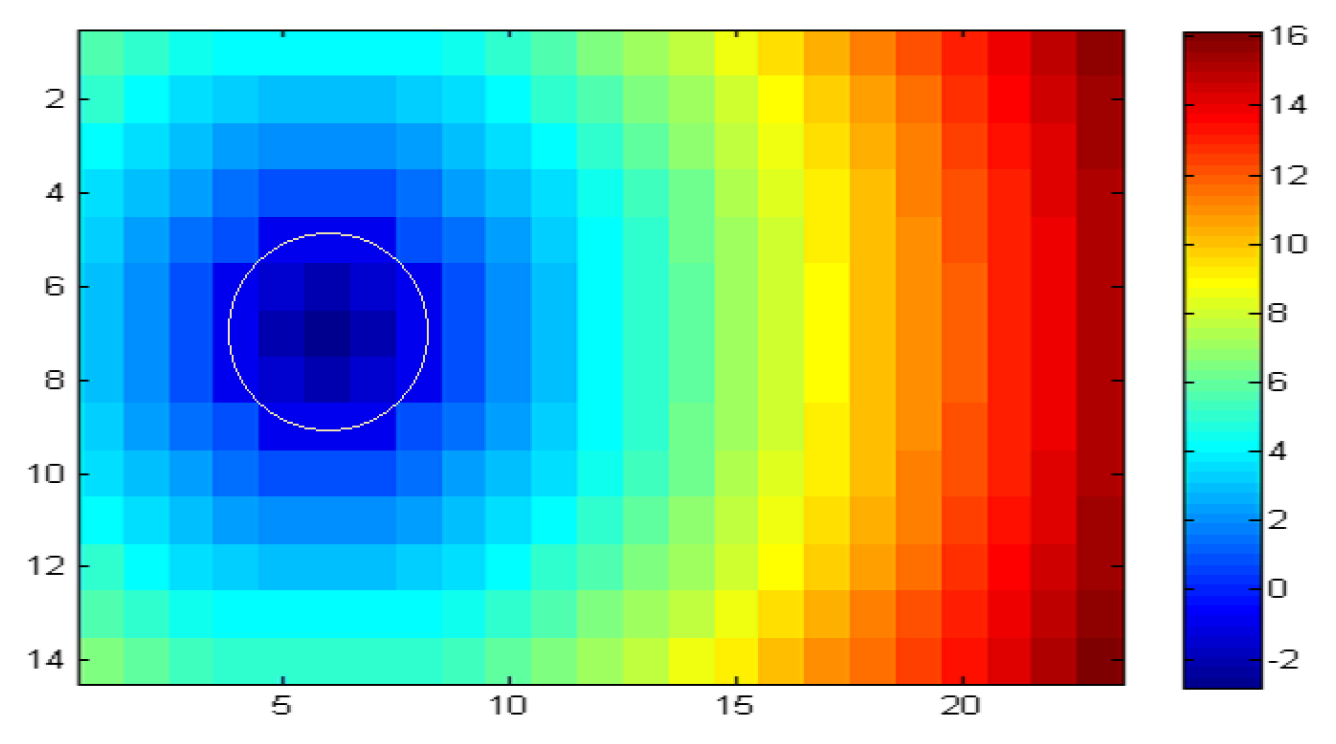
\includegraphics[width=0.54\textwidth]{figures/sdf.png}
	\caption{SDF原理示意图}
	\label{fig:sdf}
\end{figure}

$D(i, j)$表示给定点$(i, j)$到几何边界的最短距离。
图\ref{fig:sdf}是利用SDF表示二维几何图形的示意图。表示的几何图形使用白线表示,形状为圆形。


\textbf{二元法}~~图\ref{fig:binary}是二元法原理示意图,先将几何图形投射到笛卡尔网格上,使用$B(i, j)$表示二元法,则当点在几何体内部或边界时,$B(i, j) = 1$,当点在几何体外部时,$B(i, j) = 0$,通过这样表示就能将几何图形表示为一张“人工图像”。
相对于SDF,二元法进行了进一步简化,每个点到边界的物理距离没有显示的表示出来,但是对于图像数据而言,我们认为每个点的位置信息都在坐标信息中有所体现。因此,从简化预处理的角度出发,实验中使用了二元法对流场边界条件和几何图形进行表示。

\begin{figure}[htp]
	\centering
	%\includegraphics[width=0.42\textwidth]{data/MLP.pdf}
	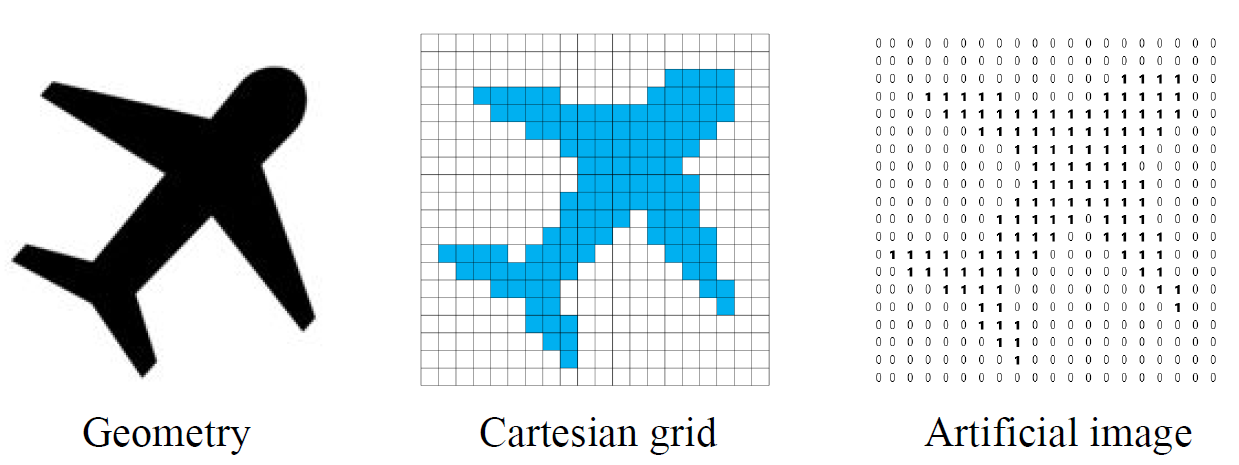
\includegraphics[width=0.64\textwidth]{figures/binary.png}
	\caption{二元法原理示意图}
	\label{fig:binary}
\end{figure}


无论是SDF和二元法,在输入流场时表示的边界条件和几何图形,在模型完成训练后进行流场预测时,每个笛卡尔网格点上的数值就不再表示几何图形,而是预测的物理量。通常输出特征图大小与输入相同,不同维度的特征图分别表示不同物理量在流场中的分布。




\section{基于U-net网络的气动流场预测}



\subsection{稳态流场预测深度模型(\textsc{FlowDNN})}
本章基于U-net网络优化设计了专用于稳态流场预测的深度神经网络架构\textsc{FlowDNN},
图\ref{fig:flowdnn}展示了\textsc{FlowDNN}网络结构。


\begin{figure}[htp]
	\centering
	%\includegraphics[width=0.42\textwidth]{data/MLP.pdf}
	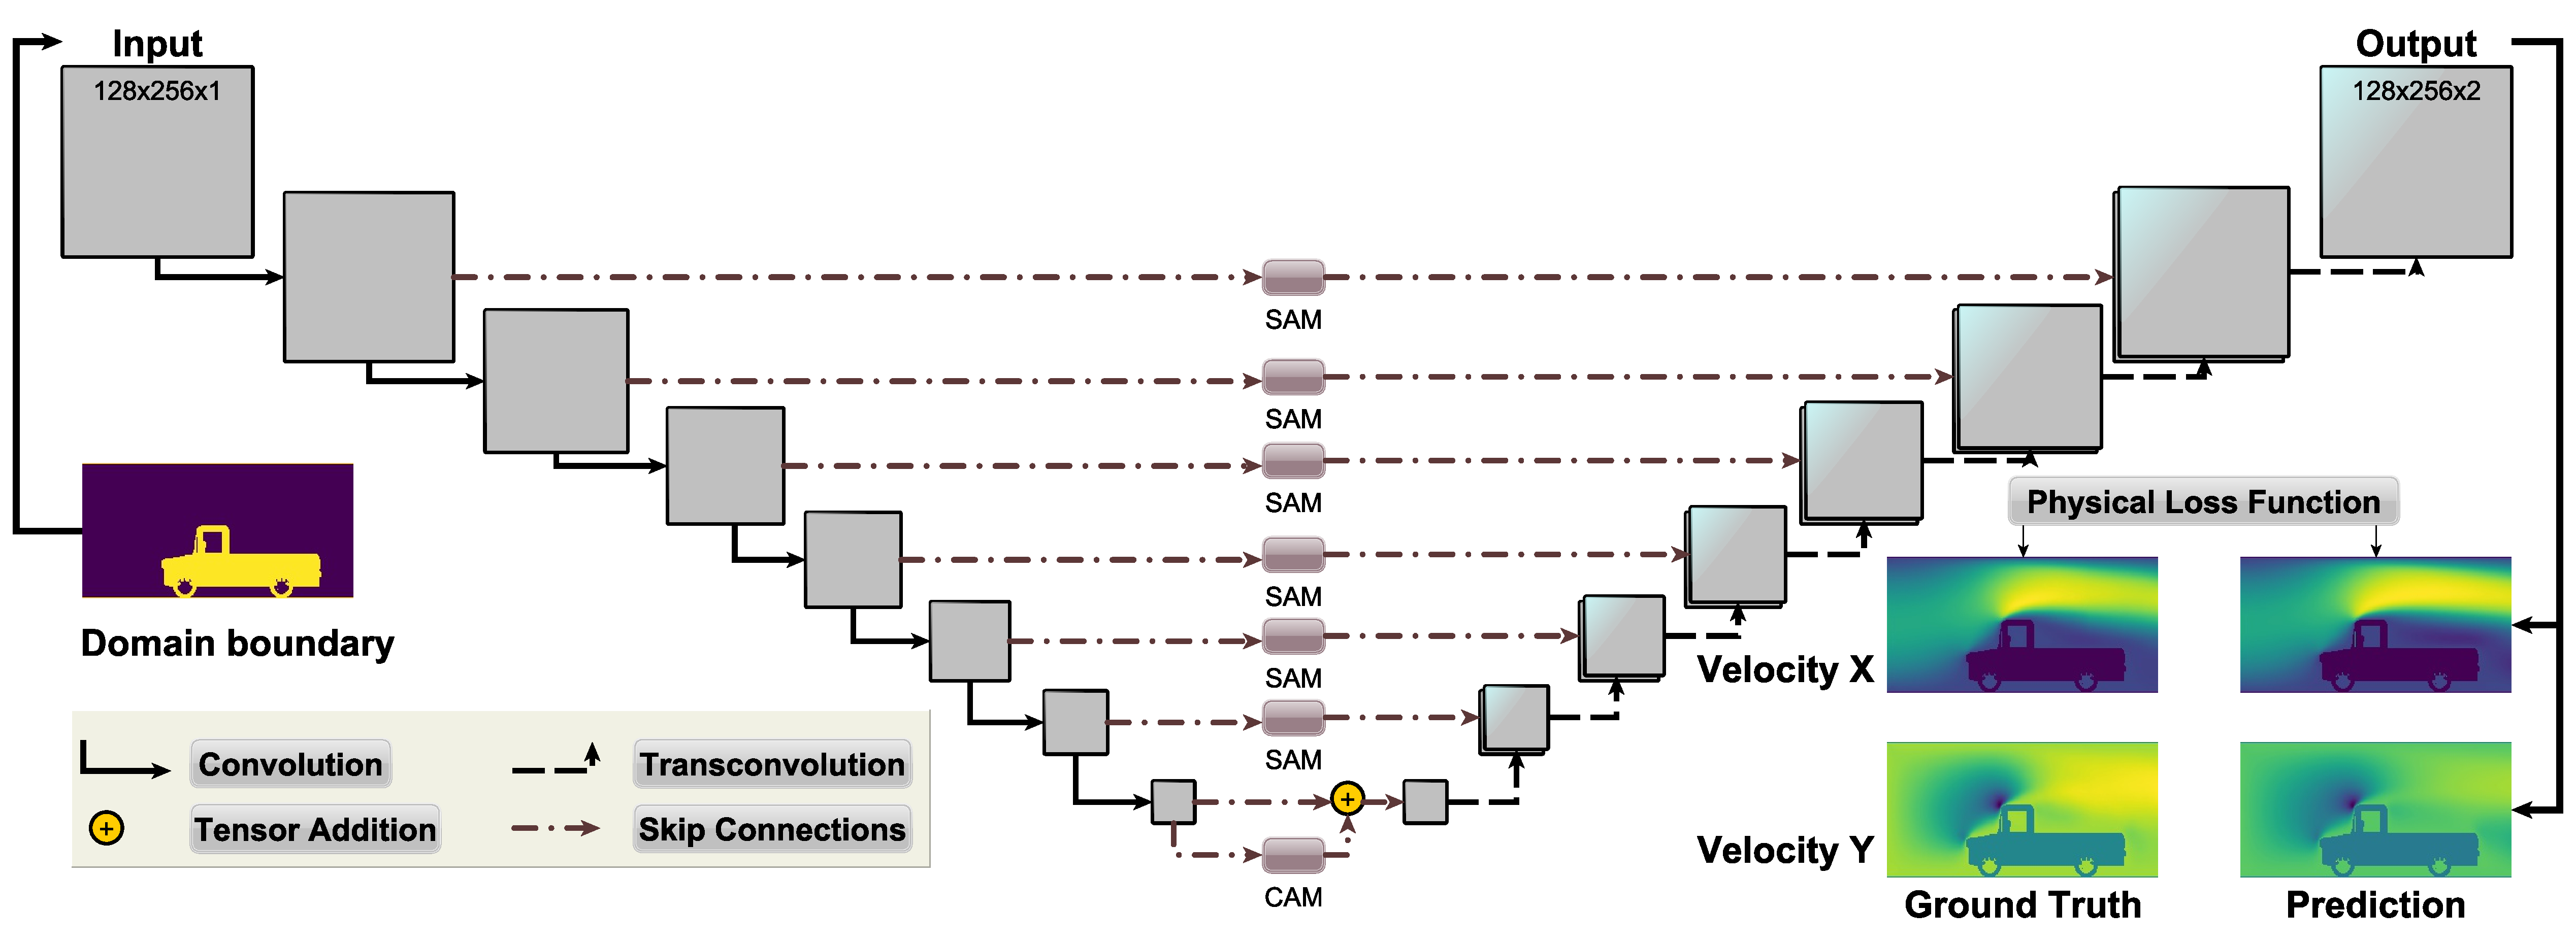
\includegraphics[width=0.99\textwidth]{figures/data/architecture.pdf}
	\caption{\textsc{FlowDNN}网络结构示意图}
	\label{fig:flowdnn}
\end{figure}

\noindent 黑色实线箭头表示卷积层和黑色虚线箭头表示反卷积层,棕色箭头表示嵌入注意力模块的skip connection。
流场边界和几何外形经过预处理得到“人工图像”作为网络输入。 输出是预测的二维速度场,
预测值和真值的损失函数为物理损失函数,用于神经网络反向传播。


\begin{table}[htp]
	\caption{
		\textsc{FlowDNN}的网络结构细节}
	\centering
	\begin{tabular}{p{3cm}p{3cm}p{3cm}p{3cm}}
		\toprule[0.4mm]
		& \multicolumn{1}{l}{编码部分} & \multicolumn{1}{l}{解码部分} \\
		\midrule
		
		\textit{Input}   & 128 x 256 x 1	& 1 x 2 x 128    \\
		\midrule
		\textit{(DE)CONV1}   &	4 x 4, 16, 2	& 2 x 2, 128, 2      	\\
		\textit{(DE)CONV2}   &	4 x 4, 32, 2	& 4 x 4, 128, 2    	\\
		\textit{(DE)CONV3}   &	4 x 4, 32, 2	& 4 x 4, 64, 2      \\
		\textit{(DE)CONV4}   &	4 x 4, 64, 2	& 4 x 4, 64, 2      \\
		\textit{(DE)CONV5}   &	4 x 4, 64, 2	& 4 x 4, 32, 2      \\
		\textit{(DE)CONV6}   &	4 x 4, 128, 2	& 4 x 4, 32, 2      \\
		\textit{(DE)CONV7}   &	2 x 2, 128, 2	& 4 x 4, 2, 2      \\

		\midrule
		\textit{Output}   & 	1 x 2 x 128		& 128 x 256 x 2      \\
		%		Ours w/ AM \& $P^2$		&\textbf{5.20\%}  & \textbf{1.99}   	& 8.50   \\
		\bottomrule[0.4mm]
	\end{tabular}
	\label{tab:flowdnn}
\end{table}

表\ref{tab:flowdnn}展示了\textsc{FlowDNN}网络结构的具体细节。
对于输入和输出而言,128 x 128 x 1表示只有1个通道且大小为128x128的特征图。
对于(逆)卷积层来说,4 x 4表示卷积核的大小,16表示卷积核的数量,2表示步长。
作为U-net的变体,\textsc{FlowDNN}也具有“U”形架构,包括7个下采样模块和7个上采样模块分别用于编码和解码。
每个下采样模块包括一个卷积层,一个激活层和一个批标准化层;卷积核的填充(padding)为1,步长为2,
用来实现下采样以提取高维抽象特征。
由于使用了逆卷积操作,可能会使预测结果出现棋盘效应\cite{odena2016deconvolution},影响预测的精度。
所以为了消除棋盘效应的影响,本文卷积核大小设置为步长2的整数倍,而不是常用的3x3或者5x5等尺寸。
前六个卷积核的感受视野为4x4,最底部的卷积核大小为2x2,因为此时输入特征图大小仅为1x2(填充之后为3x4)。
上采样层结构类似,不同的是使用逆卷积操作进行特征图的扩展,且不再使用批标准化。
每个下采样模块和上采样模块通过skip connection连接。
为了更好的融合浅层的特征,本文在skip connection上嵌入了注意力模块(细节参考\ref{注意力}节)
,增加模型的非线性和学习能力,加强不同维度信息的交互。



\subsection{物理损失函数}
将气动流场预测问题转化为图像回归预测问题后,在深度学习中常使用均方误差或均方根误差等损失函数来指导模型训练,
使预测结果在每个像素点上尽可能接近真值。
考虑到流体运动遵循一定的流动规律,仅仅依靠传统的$L_1$或$L_2$损失函数来约束神经网络训练,
可能会导致模型给出的误差较低但是不符合物理规律的预测结果。
因此,本文基于流体流动的物理规律,提出了融合物理损失项和传统$L_1$损失项的物理损失函数,
以“软”约束的方式,指导模型训练,在保证预测结果准确率的前提下,得到满足物理一致性的结果。
对于二维定常不可压流体流动问题,其宏观控制方程可以简化为:

\begin{align}
	\frac{\partial u}{\partial x}+\frac{\partial v}{\partial y}=0 
	\label{mass}\\
	\frac{\partial(u u)}{\partial x}+\frac{\partial(u v)}{\partial y}=\frac{\partial \tau_{x x}}{\partial x}+\frac{\partial \tau_{y x}}{\partial y}-\frac{\partial p}{\partial x} 
	\label{momentu1}\\
	\frac{\partial(v u)}{\partial x}+\frac{\partial(v v)}{\partial y}=\frac{\partial \tau_{x y}}{\partial x}+\frac{\partial \tau_{y y}}{\partial y}-\frac{\partial p}{\partial y} 
	\label{momentu2}\\
	e_{i n}+\frac{u^{2}+v^{2}}{2}=e \label{energy}
\end{align}

\noindent 其中方程\ref{mass}是根据质量守恒定律定义的连续性方程,方程\ref{momentu1}和\ref{momentu2}是根据牛顿第二定义的动量方程(x方向和y方向动量分量均守恒),方程\ref{energy}是在不考虑源项和扩散项的条件下得到的能量守恒方程。
具体而言,$u$和$v$分别代表x方向和y方向的速度分量,$\tau _{xx}$,$\tau _{yx}$,$\tau _{xy}$和$\tau _{yy}$
是粘性应力张量, $p$表示压力,${e_{in}}$是单位质量物质的内能,$e$是单位质量物质的总能量。
本文不考虑能量守恒方程并忽略了压力场的作用,依据连续性方程和动量守恒方程并结合传统深度学习训练中的损失函数$L_1$设计了新的物理损失函数:

\begin{align}
	L_{{\rm{physical}}} = {\alpha _1}{L_1} + {\alpha _2}{L_{{\rm{mass}}}} + {\alpha _3}{L_{{\rm{momentum}}}}
\end{align}
\noindent 其中${\alpha _1}$,${\alpha _2}$和${\alpha _3}$是三个损失项的权重。
对于二维几何有:

\begin{align}
	{{L_1} = \frac{1}{{2m{n_x}{n_y}}}\sum\limits_{l = 1}^m {\sum\limits_{i = 1}^{{n_x}} {\sum\limits_{j = 1}^{{n_y}} {\left( {\left| {u_{ij}^l - \overline u _{ij}^l} \right| + \left| {v_{ij}^l - \overline v _{ij}^l} \right|} \right)} } } }
\end{align}

\begin{align}
	\begin{array}{*{20}{c}}
		{{L_{{\rm{mass}}}} = \frac{1}{{m\left( {{n_x} - 2} \right)\left( {{n_y} - 2} \right)}}\sum\limits_{l = 1}^m {\sum\limits_{i = 2}^{{n_x} - 1} {\sum\limits_{j = 2}^{{n_y} - 1} {} } } } 
		{\left| {\left( {\frac{{\partial u}}{{\partial x}} + \frac{{\partial v}}{{\partial y}}} \right)_{ij}^l - \left( {\frac{{\partial \overline u }}{{\partial x}} + \frac{{\partial \overline v }}{{\partial y}}} \right)_{ij}^l} \right|}  
	\end{array}
\end{align}

\begin{align}
	\begin{array}{*{20}{c}}
		{{L_{{\rm{momentum}}}} = \frac{1}{{m\left( {{n_x} - 2} \right)\left( {{n_y} - 2} \right)}}\sum\limits_{l = 1}^m {\sum\limits_{i = 2}^{{n_x} - 1} {\sum\limits_{j = 2}^{{n_y} - 1} {} } } }  \\
		{\left\{ {\left| {\left[ {\left( {\frac{{\partial (uu)}}{{\partial x}} + \frac{{\partial \left( {uv} \right)}}{{\partial y}}} \right)_{ij}^l - \frac{1}{{{\mathop{\rm Re}\nolimits} }}\left( {\frac{{{\partial ^2}u}}{{\partial {x^2}}} + \frac{{{\partial ^2}u}}{{\partial {y^2}}}} \right)_{ij}^l} \right] - } \right.} \right.}  
		{\left. {\left[ {\left( {\frac{{\partial (\overline u \overline u )}}{{\partial x}} + \frac{{\partial \left( {\overline u \overline v } \right)}}{{\partial y}}} \right)_{ij}^l - \frac{1}{{{\mathop{\rm Re}\nolimits} }}\left( {\frac{{{\partial ^2}\overline u }}{{\partial {x^2}}} + \frac{{{\partial ^2}\overline u }}{{\partial {y^2}}}} \right)_{ij}^l} \right]} \right| + }  \\
		{\left| {\left[ {\left( {\frac{{\partial (vu)}}{{\partial x}} + \frac{{\partial \left( {vv} \right)}}{{\partial y}}} \right)_{ij}^l - \frac{1}{{{\mathop{\rm Re}\nolimits} }}\left( {\frac{{{\partial ^2}v}}{{\partial {x^2}}} + \frac{{{\partial ^2}v}}{{\partial {y^2}}}} \right)_{ij}^l} \right]} \right. - }  
		{\left. {\left. {\left[ {\left( {\frac{{\partial (\overline v \overline u )}}{{\partial x}} + \frac{{\partial \left( {\overline v \overline v } \right)}}{{\partial y}}} \right)_{ij}^l - \frac{1}{{{\mathop{\rm Re}\nolimits} }}\left( {\frac{{{\partial ^2}\overline v }}{{\partial {x^2}}} + \frac{{{\partial ^2}\overline v }}{{\partial {y^2}}}} \right)_{ij}^l} \right]} \right|} \right\}}  
	\end{array}
\end{align}

\noindent 其中$m$是神经网络训练中训练样本批大小(batch size),$l$表示某个样本,
$n_x$和$n_y$是沿x方向和y方向的像素(网格)数量,
$u$和$v$分别是x方向和y方向的速度分量,$\overline u$和$\overline v$
代表相应方向上的预测速度分量。
$L_{\rm {mass}}$是基于质量守恒定律的损失函数,
评估在预测流场和参考流场(由CFD求解器计算得到,即深度学习训练中的真值)中每个单元质量变化的差异。
同理,$L_{\rm {momentum}}$是基于动量守恒定律的损失函数,
比较预测流场和参考流场中x和y方向上的动量变化的差异。 
\textit{Re}代表固定的雷诺数(Reynolds number),
流动条件通常通过描述惯性比的无量纲雷诺数来量化,以区分是否为有粘流动问题。
在这里,一阶和二阶偏导数是使用
一阶和二阶中心差分格式\cite{blazek2015computational},以x方向的速度$u$为例有:

\begin{align}
	\small
	\begin{array}{*{20}{c}}
		{\frac{{\partial {u_{i,j}}}}{{\partial x}} = \frac{1}{2}\left( {{u_{i + 1,j}} - {u_{i - 1,j}}} \right)};\\
		{\frac{{{\partial ^2}{u_{i,j}}}}{{\partial {x^2}}} = {u_{i + 1,j}} - 2{u_{i,j}} + {u_{i - 1,j}}}  \\
	\end{array}
\end{align}


\subsection{注意力机制}\label{注意力}
在计算机视觉中图像分割或者目标检测等任务中,研究者通常希望网络能够更多的关注一些特定的区域,比如目标所在的区域,注意力机制\cite{Hu2017Squeeze}是常用的优化方法之一。
类似地,在气动流场预测任务中,也有类似的需求。CFD研究者通常更加关注几何体周围的流场,这部分区域一般称为感兴趣区域(Region of  Interest,RoI)。原因是这部分区域流场变化快,蕴含的信息多,一些关键的气动系数(如升阻比,压力系数等)也与几何体周围的流场更相关。
经过以上分析,我们在气动流场预测网络结构中引入注意力机制,期望能够提升RoI区域的预测精度。

\textsc{FlowDNN}嵌入了两个轻量级注意力模块:通道注意力模块(channel attention module,CAM)和空间注意力模块(spatial attention module,SAM)\cite{DBLP:conf/eccv/WooPLK18}。
CAM和SAM分别可以从通道维度和空间维度自适应提取神经网络需要重点关注的信息,
图\ref{fig:am机制}是CAM和SAM的结构示意图。

\begin{figure}[htp]
	\centering
	%\includegraphics[width=0.42\textwidth]{data/MLP.pdf}
	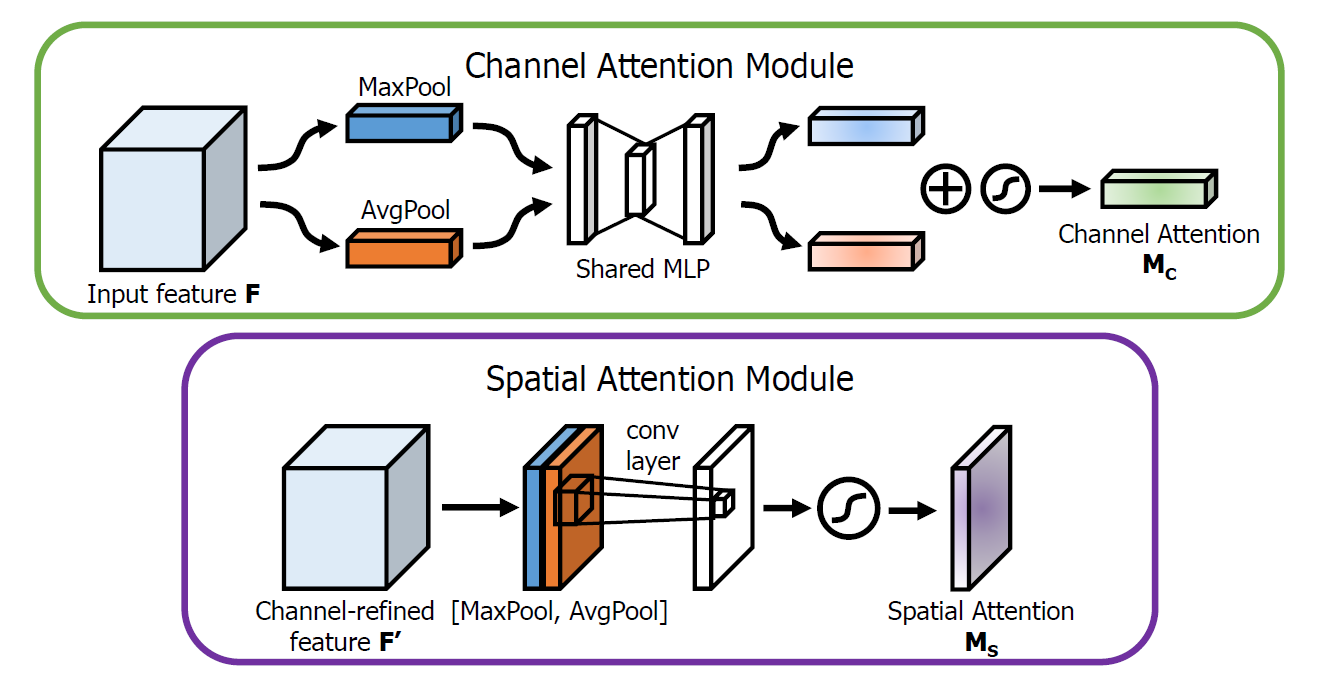
\includegraphics[width=0.88\textwidth]{figures/am.png}
	\caption{CAM和SAM结构示意图\cite{DBLP:conf/eccv/WooPLK18}}
	\label{fig:am机制}
\end{figure}

CAM通过全局池化操作和多层感知机对通道维度的信息进行了整合,
SAM通过全局池化操作和卷积操作对空间维度的信息进行了整合,具体工作原理如下:
\begin{align}
\mathbf{F}_{\mathbf{c}} &=\mathbf{M}_{\mathbf{c}}(F) \otimes F \\
\mathbf{F}_{\mathbf{s}} &=\mathbf{M}_{\mathbf{s}}\left(F\right) \otimes F \\
\mathbf{M}_{\mathbf{c}}(F) &=\mathbf{\sigma}(\mathbf{MLP}(\mathbf{GAP}(F))+\mathbf{MLP}(\mathbf{GMP}(F))) \label{eq8}\\
\mathbf{M}_{\mathbf{s}}(F) &=\mathbf{\sigma}\left(Conv\left(\mathbf{GAP}_\mathbf{c}\left(F\right) \oplus \mathbf{GMP}_\mathbf{c}\left(F\right)\right)\right) \label{eq9}
\end{align}

\noindent 其中$F \in R^{C \times H \times W}$表示输入特征图(C、H、W分别表示通道数和特征图的高度及宽度),
$\mathbf{M}_{\mathbf{c}} \in R^{C \times 1 \times 1}$和$\mathbf{M}_{\mathbf{s}} \in R^{1 \times H \times W}$
分别代表CAM和SAM。
$\otimes$表示元素乘法,经CAM和SAM处理后的输出特征图$\mathbf{M}_{\mathbf{c}}(F)$和$\mathbf{M}_{\mathbf{s}}\left(F\right)$
需要与输入特征图$F$相乘,保证输入和最终输出的大小和维度一致。
公式\ref{eq8}和\ref{eq9}展示了CAM和SAM的具体操作:
CAM先对输入特征图在空间域进行全局最大池化(global  max pooling,GMP)和全局平均池化(global average pooling,GAP),分别得到一个单通道向量,
再将该向量输入一个多层感知机进行通道方向的信息融合,最后将GMP和GAP的结果相加,
通过sigmoid激活函数得到$\mathbf{M}_{\mathbf{c}}(F)$;
SAM也对输入特征图进行了GMP和GAP,不同的是池化操作是在通道方向进行;
利用$\oplus$操作,将池化的结果进行叠加,然后利用卷积操作对空间维度的信息进行融合。

由于SAM模块中含有卷积操作,神经网络剪枝会对SAM模块产生影响,
所以在设置注意力模块时仅在“U”形\textsc{FlowDNN}的底部设置了SAM模块,其他skip connections仅嵌入CAM模块;
在进行神经网络剪枝时,与SAM模块相连的卷积层和逆卷积层不参与剪枝,保证SAM模块不受影响。
CAM模块通过多层感知机进行通道维度的信息融合,因此不受神经网络剪枝的影响。


\subsection{神经网络剪枝}
神经网络剪枝(network pruning)通过裁剪卷积层中卷积核大小或数量及其关联层参数大小,
减小模型的计算量和体积,从而加快模型部署后的推理速度,是一种减小模型大小和降低模型计算复杂度的常用方式。
在气动流场预测模型训练完成后,我们对网络进行了神经网络剪枝\cite{DBLP:conf/iclr/LiuSZHD19},
主要有两方面考虑:
a)一方面,相对于基线模型\textsc{FlowDNN}的网络参数较多。通过对网络进行剪枝,
可以证明\textsc{FlowDNN}对气动流场预测性能的提升不是简单的增加网络参数量;
b)另一方面,由于神经网络的冗余性,适当的剪枝并不会对预测精度产生明显的影响,
但是剪枝后模型的推理时间将有效减少。对于复杂的大规模气动流场模拟,剪枝对于提升预测性能意义重大。

神经网络剪枝要解决的核心问题就是“剪哪里”,
即评估卷积核重要性的标准,常见的标准有:内核权重的大小,特征映射激活值的均值、标准差和比例,激活值和预测值之间的互信息等。
本文采用了文献\cite{DBLP:conf/iclr/MolchanovTKAK17}的方法,
通过基于泰勒展开的方法近似评估每个卷积核被剪枝后损失函数的变化,进而根据卷积核的重要性对网络进行裁剪。
图\ref{fig:pruning}是神经网络剪枝的流程示意图:
1)载入训练好的模型;2)通过剪枝算法对每个卷积核的重要性进行评估;3)剔除重要性最低的卷积核;
4)利用训练数据对剪枝后的网络进行微调;
5)判断网络剪枝是否满足预设条件(参数量等),如果不满足,返回第二步;如果满足就结束网络剪枝。
 

\begin{figure}[htp]
	\centering
	%\includegraphics[width=0.42\textwidth]{data/MLP.pdf}
	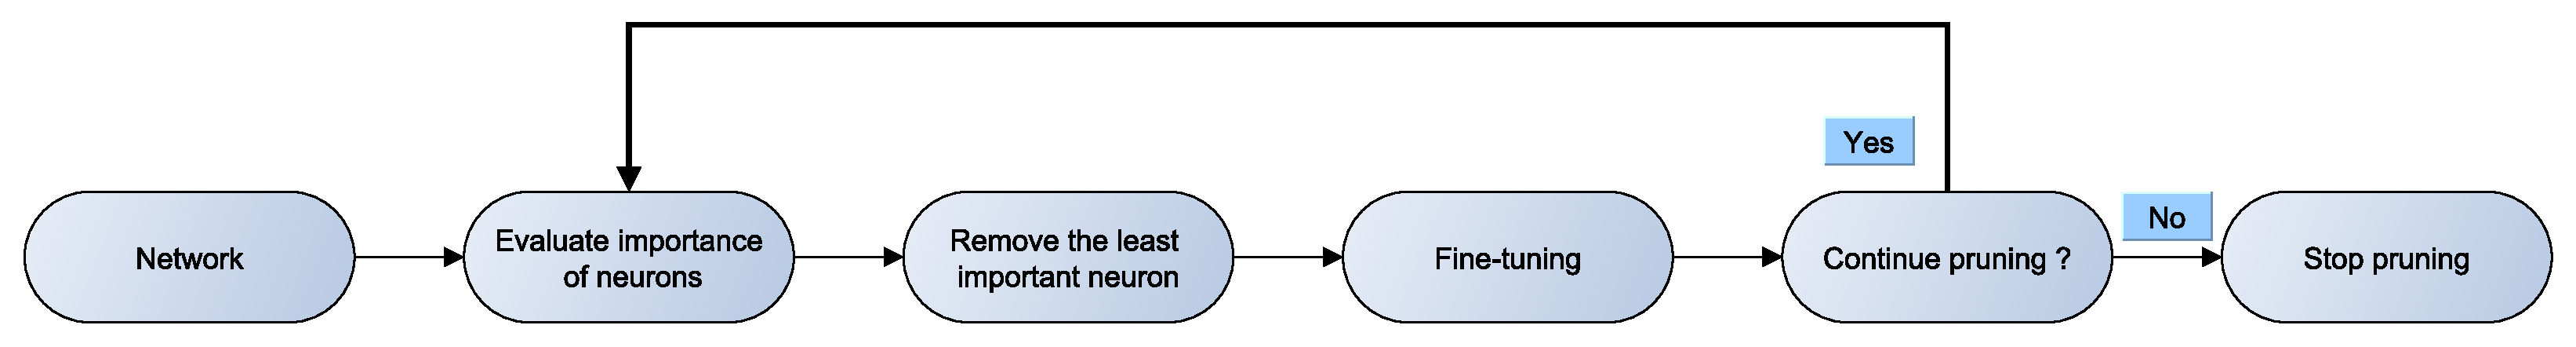
\includegraphics[width=0.99\textwidth]{figures/pruning_flow.pdf}
	\caption{神经网络剪枝流程示意图}
	\label{fig:pruning}
\end{figure}



\section{实验设置与结果分析}

\subsection{数据集与参数设置}

\subsubsection{基于LBM求解器生成数据集}
实验算例设置为二维定常不可压层流的外流问题,几何外形为不同形状的二维汽车外形。
我们使用基于LBM方法的开源库MECHSYS\footnote{ http://mechsys.nongnu.org}对二维流场进行模拟。
为了验证模型的泛化能力,我们将训练集设置为3000个简单几何体的组合形状,包括三角形、圆形、椭圆和方形等,不同样本中几何体大小和位置不同;验证集和测试集分别是22和44个不同形状的汽车外形。图\ref{fig:sample}是部分训练集样本和测试集数据样本可视化结果。

\begin{figure}[htb]
	\centering
	\subfloat[训练集]{\label{fig:training_sample}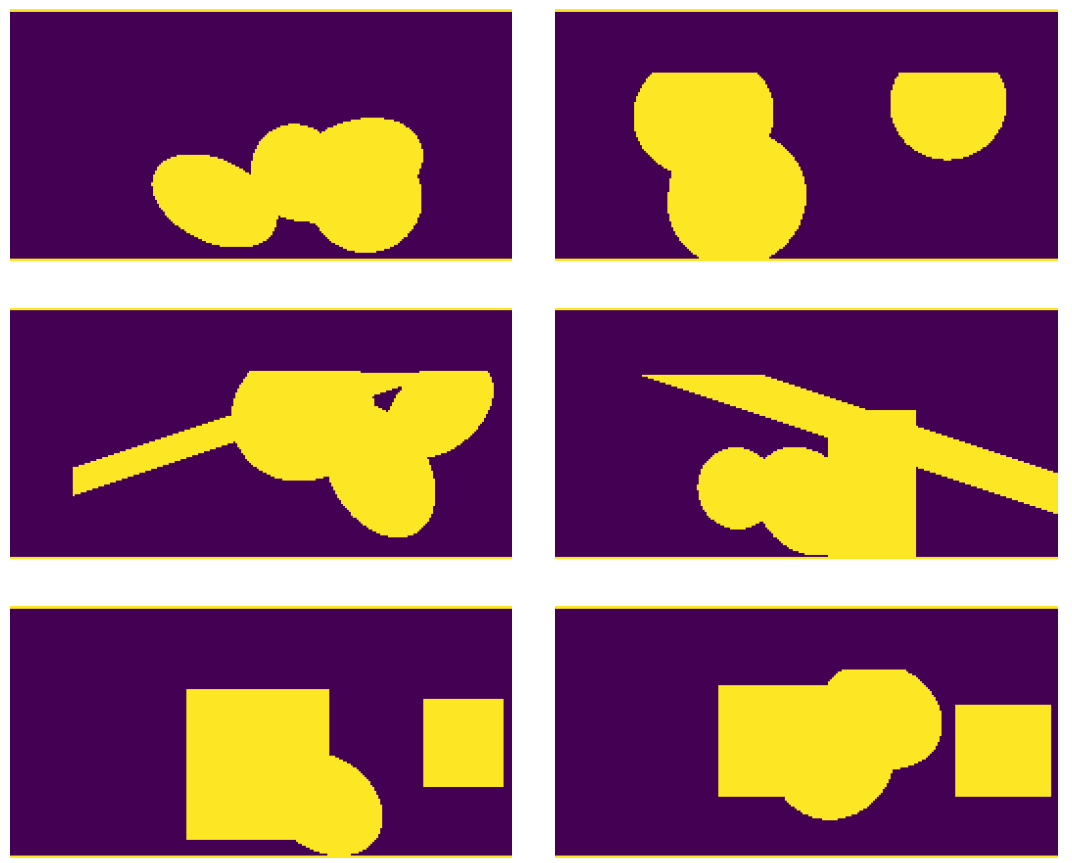
\includegraphics[width=0.42\textwidth]{figures/data/data_rep/training_sample/train_sample.png}} \qquad
	\subfloat[测试集]{\label{fig:testing_sample}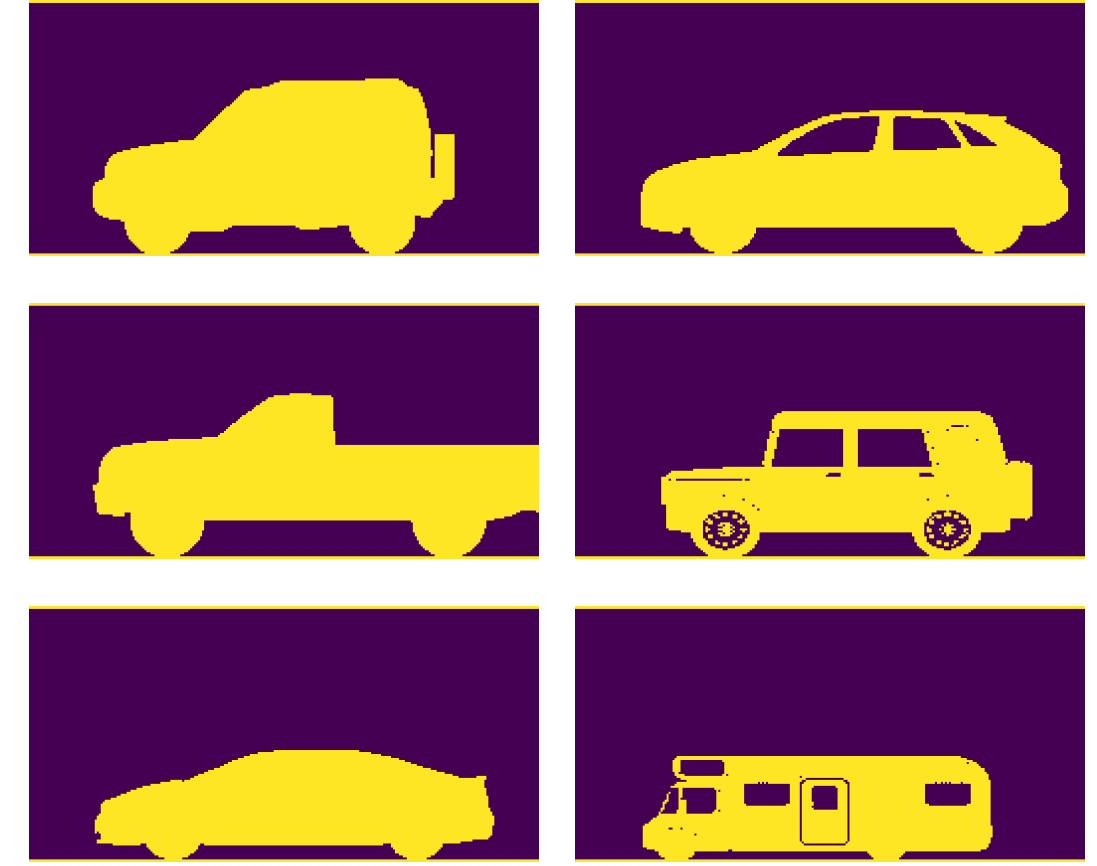
\includegraphics[width=0.42\textwidth]{figures/data/data_rep/training_sample/test_sample.png}} 
	\caption{训练集和测试集数据样本可视化示例}
	\label{fig:sample}
\end{figure}

在进行LBM流场模拟时,雷诺数设置为400以获取层流模拟结果;气流流向与x方向平行,采用D2Q9模型对速度矢量进行离散。
所有LBM求解程序都在GPU上并行执行,迭代10000时间步,保证计算结果的收敛性。
神经网络训练输入和输出特征图尺寸相同,输入为基于二元法表示的几何外形,输出为二维速度场,笛卡尔网格大小为256x128。


\subsubsection{参数设置}

\newcommand{\tabincell}[2]{\begin{tabular}{@{}#1@{}}#2\end{tabular}}
\begin{table}[htp]
	\setlength{\belowcaptionskip}{0.0cm}
	\caption{模型训练超参数设置 }
	\label{tab:parameters}
	\centering
	\begin{tabular}{p{1.9cm}p{1.6cm}p{1.2cm}p{1.4cm}p{1.6cm}p{1.2cm}p{1.4cm}}
		\toprule
		& \tabincell{c}{Learning \\ rate (Lr)}  & \tabincell{c}{Lr decay \\ interval} &  \tabincell{c}{Batch \\ size} & \tabincell{c}{Size of \\ the filters}  & \tabincell{c}{ Pruning \\ number}  & \tabincell{c}{Weights of \\ $L_{\rm{physical}}$} \\
		\midrule
		Optimum  &$4\times10^{-4}$  &	25 &	16 & 4 &1  & (1, 5, 25) $/$ 3  \\
		\midrule
		Tuning range & $10^{-5}$ \textasciitilde $10^{-3}$ 	&	20\textasciitilde 50 	&4\textasciitilde64  & 	2\textasciitilde8	 &1\textasciitilde5  &  - \\
		
		
		\bottomrule
	\end{tabular}
\end{table}

\textsc{FlowDNN}基于PyTorch深度学习框架编程实现,
在实验中,我们利用英伟达Tesla V100 GPU实现模型的训练、参数调优和神经网络剪枝。
深度学习训练有许多超参数,包括批大小学习率等,
表\ref{tab:parameters}展示了一些重要的超参数调优的范围以及最终的设置。
模型训练使用Adam优化算法,为了得到稳定收敛的结果,模型在数据集上训练400轮次(epoch)。
初始学习率设置为$4\times10^{-4}$,每25个epochs将学习率更新,乘以衰减因子0.9。
学习率衰减的好处是适应模型训练的特点,在前期加速模型训练,后期保证模型收敛至稳定状态。
批大小设置为16,意味着模型在进行推理时可以同时对16个不同初始条件流场进行预测。
在剪枝过程中,我们对每次剪枝的数量进行了探究,最终决定每次迭代只剪枝一个神经元,
因为一次剪枝过多会破坏神经网络结构,导致预测准确率急剧下降。每个剪枝迭代步之后,对剪枝后的网络进行微调,
训练40个epochs是神经网络收敛。
对激活函数,本文考虑两种常用的激活函数ReLU(rectified linear units)和ELU(exponential linear units),
其中ELU激活函数在文献\cite{DBLP:journals/corr/abs-1908-04387}中被推荐使用,两者的比较结果可见\ref{ac_effect}节。
对于损失函数的权重,我们先固定${\alpha _1}$为1,然后调整${\alpha _2}$和${\alpha _3}$使得损失函数的每一项在数值上对总的损失函数贡献相当;由于我们有损失函数有三项,将${\alpha _1}$、${\alpha _2}$和${\alpha _3}$分别除以3,即为最终损失函数的权重。




\subsubsection{性能评估标准}

\textbf{基线模型}

本文引入三个基线模型,用来比较和评估\textsc{FlowDNN}对稳态流场的预测结果:\\
(1) \texttt{C-Net}\cite{DBLP:conf/kdd/GuoLI16}:基于自编码器的流场预测方法,
	使用了3层卷积层和3层逆卷积层分别是实现对流场数据的编码与解码。\\
(2)	\texttt{T-Net}\cite{thuerey2019deep}:基于U-net改进的流场预测方法,
	基于深度神经网络推断RANS模型的流场压力场与速度场分布。\\
(3) \texttt{U-Net}\cite{DBLP:conf/miccai/RonnebergerFB15}:用于图像分割的经典深度神经网络,
	被广泛用于图像回归预测任务。

	




\textbf{流场预测结果评价指标}

对于深度神经网络模型的预测结果,本文使用平均相对误差(Mean Relative Error,MRE)比较预测流场和真值之间的差异,对气动流场的预测准确率进行总体的评估。
除了全场模拟结果,CFD领域专家通常对某些特定的区域感兴趣,比如流场边界层(即几何体表面附近流场),在RoI区域中流场变化剧烈,往往包含着更多有用的信息。对于本文使用的汽车外部流场,我们定义RoI区域如图\ref{fig:errors_area}中红色方框选中区域所示。RoI不是固定的,对于不用的汽车外形,红色方框自适应地恰好选中整个汽车。在确定了RoI之后,即可求得该区域的平均相对误差$\rm{MRE_{RoI}}$。
根据流体流动遵循的质量守恒定律和动量守恒定律,我们设计了${\rm{MRE}_{ma}}$和${\rm{MRE}_{mo}}$分别评测模型预测结果与真值的质量守恒一致性和动量守恒一致性。

\begin{figure}[htp]
	\centering
	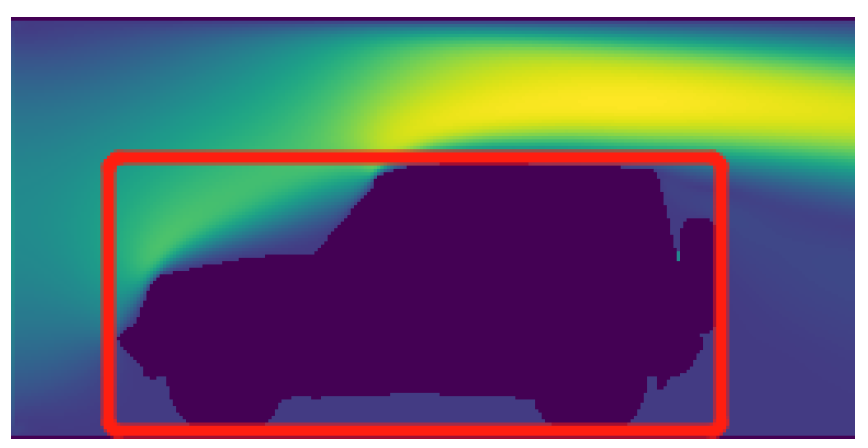
\includegraphics[width=0.44\textwidth]{figures/data/data_rep/errors.png}
	\caption{RoI示意图}	
	\label{fig:errors_area}
\end{figure}

在测试集有N个样本的情况下,对于二维流场有:
\begin{align}
MRE = { \frac{1}{N} \sum\limits_{l = 1}^N  \left( {\sum\limits_{i = 1}^{{n_x}} {\sum\limits_{j = 1}^{{n_y}} {\left( {\left| {u_{ij}^l - \overline u _{ij}^l} \right| + \left| {v_{ij}^l - \overline v _{ij}^l} \right|} \right)} } } / {{\sum\limits_{i = 1}^{{n_x}} {\sum\limits_{j = 1}^{{n_y}} {\left( {\left| {u _{ij}^l} \right| + \left| { v _{ij}^l} \right|} \right)} } }} \right) }
\end{align}

\begin{align}
MRE_{RoI} = { \frac{1}{N} \sum\limits_{l = 1}^N \left( { {\sum\limits_{i = 1}^{{n_s}} {\left( {\left|
					{u_{i}^l - \overline u _{i}^l} \right| + \left| {v_{i}^l - \overline v _{i}^l} \right|} \right)} } } /  {{ {\sum\limits_{i = 1}^{{n_s}}
				{\left( {\left| {u _{i}^l} \right| + \left| { v _{i}^l} \right|} \right)} } }} \right)}
\end{align}

\begin{align}
MRE_{ma} / MRE_{mo} = { \frac{1}{N} \sum\limits_{l = 1}^N  \left({\sum\limits_{i = 1}^{{n_x}} {\sum\limits_{j = 1}^{{n_y}} { {\left| {g_{ij}^l - \overline g _{ij}^l} \right| } } } } /  {{\sum\limits_{i =1}^{{n_x}} {\sum\limits_{j = 1}^{{n_y}} { {\left| {g _{ij}^l} \right|} } } }} \right)} 
\label{eq:mam}
\end{align}

\noindent 其中$n_s$表示在RoI中的格子数。在公式\ref{eq:mam}中,$g$和$\overline g$分别表示在真值和预测结果的每个格子点上质量(或动量)的变化值。



\subsection{实验结果与分析}

\subsubsection{总体预测性能比较}
通过大量实验,我们将基于不同深度学习方法的预测结果和基于LBM方法的求解器模拟结果进行了对比。
表\ref{tab:all_comp}展示了\textsc{FlowDNN}和基线模型在测试集上预测准确率,推理时间和模型参数量等方面的性能表现,其中AM表示嵌入了注意力模块,$P$代表神经网络剪枝;\textsc{FlowDNN}均使用物理损失函数进行训练。

\begin{table}[htp]
	\caption{不同深度学习方法的各项性能指标比较}
	
	\label{tab:all_comp}
	\centering
	
	\begin{tabular}{p{3.5cm}p{1.1cm}p{1.3cm}p{1.2cm}p{1.2cm}p{1.2cm}p{1.5cm}}
		\toprule
		\textbf{Method}  & \textbf{MRE} &  ${\textbf{MRE}_{RoI}}$ & $\textbf{MRE}_{ma}$ & $\textbf{MRE}_{mo}$ & \textbf{Runtime (ms)} & \textbf{Parameters (Mb)}\\
		\midrule
		LBM 				&	- &	-&	-&	-		&  3300$\times$16 	& -\\
		\textit{C-Net}   &	14.31\%&	30.99\% &	37.44\%&	45.60\%	&9.29    	& 180.25\\
		\textit{T-Net}   		&	24.65\%&	59.71\%&	79.09\%&	82.38\%	&  8.47 	& 7.45   \\
		\textit{U-Net}   &	14.74\%&	13.14\%&	30.78\%&	44.42\%	& 16.15      	&  32.96 \\
		\textsc{FlowDNN}   		&	7.91\%&	23.56\%& 18.28\%&	22.46\%	& \textbf{3.52}	& 13.70   \\
		\textsc{FlowDNN} w/ AM   		&5.34\% &9.16\% & 12.34\% & 15.69\%  & 4.51   	& 13.74   \\
		\textsc{FlowDNN} w/ AM \& $P$		&\textbf{4.77\%} &\textbf{8.87\%}&\textbf{12.14\%}&\textbf{14.63\%}  & \textbf{3.62}   	& \textbf{7.40}   \\
		%		Ours w/ AM \& $P^2$		&\textbf{5.20\%}  & \textbf{1.99}   	& 8.50   \\
		\bottomrule
	\end{tabular}
	
\end{table}

在模型参数量方面,因为\texttt{C-Net}网络架构中使用了全连接层,每个神经元与其前一层的所有神经元进行全连接,导致网络参数量远大于其他模型,大小为180.25Mb。
在基线模型中,\texttt{T-Net}模型参数量最小为7.45Mb,约是剪枝之前\textsc{FlowDNN}模型大小的一半。
此外,在\textsc{FlowDNN}嵌入注意力模块之后,模型大小几乎没有改变,体现出轻量级注意力模块的灵活性。
在推理时间方面,在利用深度学习模型进行流场预测时我们将批大小设置为16,即一次推理过程可以得到16个算例的预测结果。
对于每个算例,LBM求解器通过迭代计算求解控制方程得到收敛的二维速度场结果,在GPU测试平台上程序的平均运行时间约为3300ms。
对于深度学习预测模型,尽管\texttt{U-Net}模型参数不是最大,但推理时间最长,这可能和网络中卷积核的大小和采样的方式方式有关。
\textsc{FlowDNN}的推理时间最短为3.52ms,在嵌入注意力模块之后推理时间增加了近四分之一,经过神经网络剪枝后推理时间基本和嵌入注意力模块之前相当。

对于指标$MRE$和$MRE_{RoI}$,模型的预测结果基本上是$MRE_{RoI}$远大于$MRE$,
说明对于气动流场而言,几何体表面附近相较于远场更难以预测,反映出该区域速度变化更加剧烈,这符合流体流动的一般特点。
然而我们观察到\texttt{U-Net}对于全场和RoI区域的预测性能接近甚至在RoI区域更准确,这一结果可能和\texttt{U-Net}的网络结构相关,但具体的原因需要进一步探究。
相较于三种基线模型,在不引入注意力机制和神经网络剪枝的情况下,使用物理损失函数训练\textsc{FlowDNN}可以使$MRE$降低至7.91\%,接近三种基线模型中表现最好的\texttt{C-Net}的一半。
但是\textsc{FlowDNN}对RoI区域的预测效果并不理想,$MRE_{RoI}$仅为23.56\%,不仅远大于\texttt{U-Net}的13.14\%,而且是$MRE$预测误差的三倍。因此,本文引入了注意力机制希望能提升\textsc{FlowDNN}对几何体表面附近流场的预测效果。



对于指标$MRE_{ma}$和$MRE_{mo}$,不同深度学习方法的预测结果均体现出$MRE_{mo}$大于$MRE_{ma}$的趋势,可以得知相较于质量守恒,预测结果往往更难以保证动量守恒的一致性。由于\textsc{FlowDNN}均是使用物理损失函数训练,所以与基线模型相比,$MRE_{ma}$和$MRE_{mo}$误差比较小。关于损失函数对预测结果的影响可见\ref{phy_effect}节。此外,注意力模块也有效降低了$MRE_{ma}$和$MRE_{mo}$误差。



\begin{figure}[htp]
	\centering
	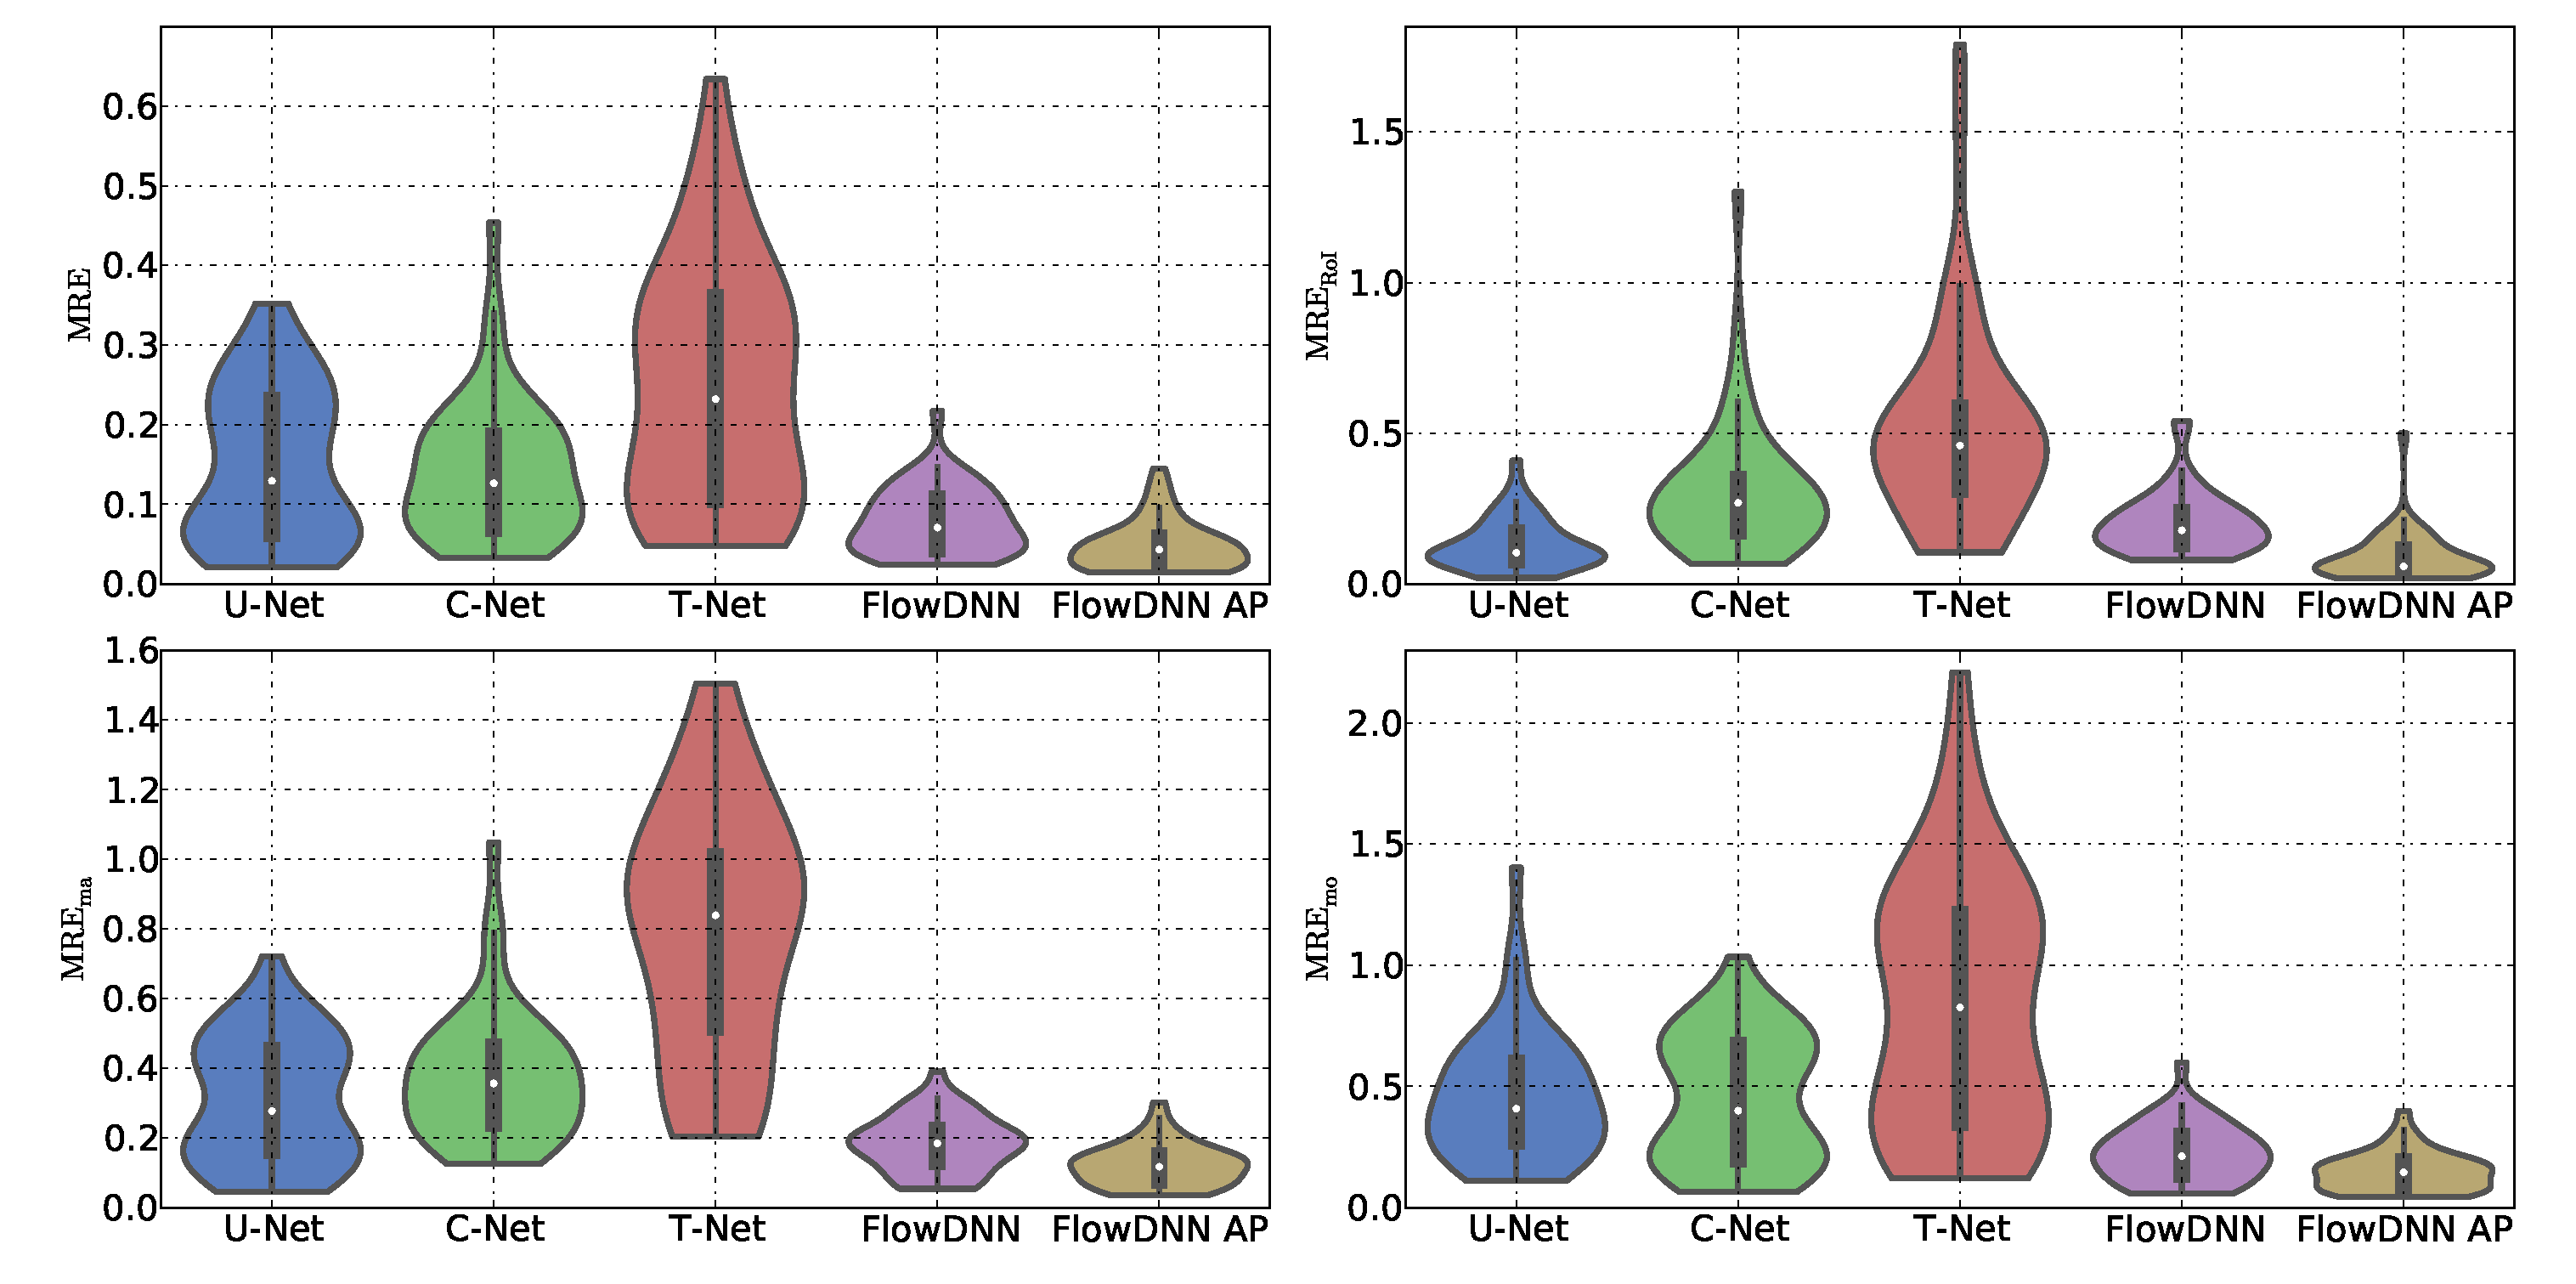
\includegraphics[width=0.98\textwidth]{./figures/data/all_violin.pdf}
	\caption{不同深度学习方法的预测性能指标在测试集上的分布}
	\label{fig:overall_violin}
\end{figure}


图\ref{fig:overall_violin}展示了$MRE$、$MRE_{RoI}$、$MRE_{ma}$和$MRE_{mo}$四种指标在测试集上分布情况。
小提琴图外围的曲线宽度代表数据点分布的密度,内部的黑色长条表示中间二分之一的样本分布的范围,白点表示所有样本的中位数。
观察三种基线模型的预测结果分布,除了\textit{U-Net}在指标$MRE_{RoI}$上表现比较稳定之外,
其他情况的预测误差都表现出很大的波动,即在某些样本上模型预测性能较好,在另一些样本上预测性能则较差,
比如\textit{U-Net}对某个算例的预测结果的$MRE$误差甚至超过了50\%。
相比之下,\textsc{FlowDNN}不仅在各项性能指标上平均误差较小,而且表现出良好的预测稳定性,对于测试集上不同的算例,
\textsc{FlowDNN}能将流场预测结果的误差控制在较小的范围。

\begin{table}[htp]
	\caption{不同深度学习方法的二维速度场预测结果}
	
	
	\label{tab:total_comp_case}
	\centering
	\begin{tabularx}{14cm}{p{0.8cm}p{1.9cm}p{1.5cm}p{1.5cm}p{1.5cm}p{1.5cm}p{2.6cm}}
		\toprule
		& ~~~~~~~LBM  & ~~~~\textit{U-Net} & ~~~~\textit{C-Net} & ~~~~\textit{T-Net} & ~~\textsc{FlowDNN} & ~~\textsc{FlowDNN} AP   \\
		\midrule
		
		racing &\multicolumn{6}{l}{
			\begin{minipage}{\textwidth}
				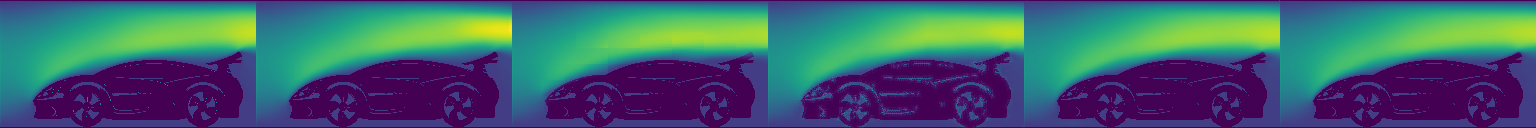
\includegraphics[width=0.82\textwidth]{./figures/data/pic_xin/final_35.png}
			\end{minipage}}
			\\
			
			saloon &\multicolumn{6}{l}{
				\begin{minipage}{\textwidth}
					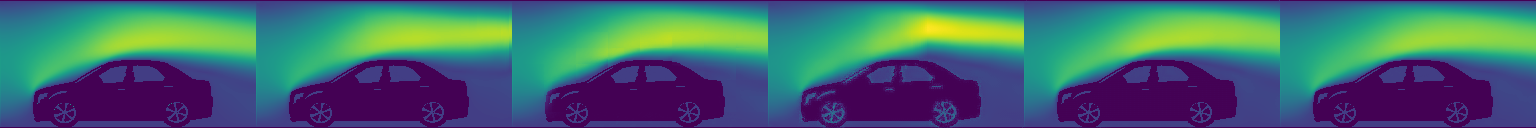
\includegraphics[width=0.82\textwidth]{./figures/data/pic_xin/final_32.png}
				\end{minipage}}
				\\
				jeep &\multicolumn{6}{l}{
					\begin{minipage}{\textwidth}
						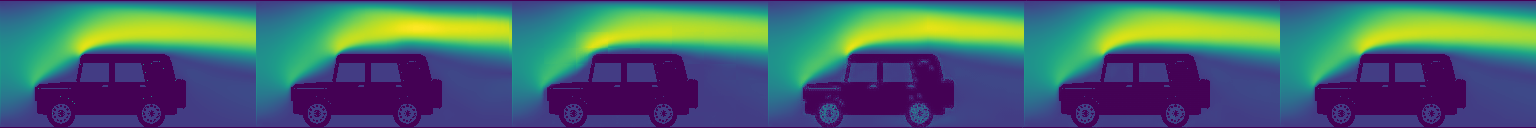
\includegraphics[width=0.82\textwidth]{./figures/data/pic_xin/final_20.png}
					\end{minipage}}
					\\
					pickup &\multicolumn{6}{l}{
						\begin{minipage}{\textwidth}
							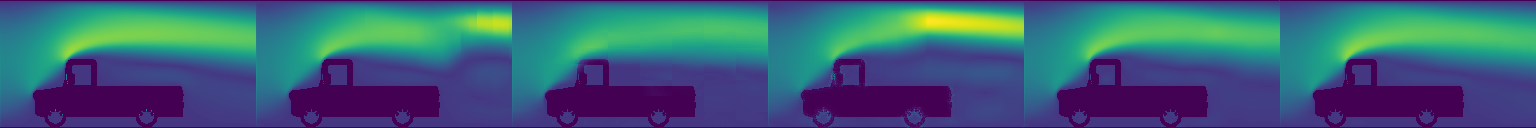
\includegraphics[width=0.82\textwidth]{./figures/data/pic_xin/final_39.png}
						\end{minipage}}
						\\	
						bus &\multicolumn{6}{l}{
							\begin{minipage}{\textwidth}
								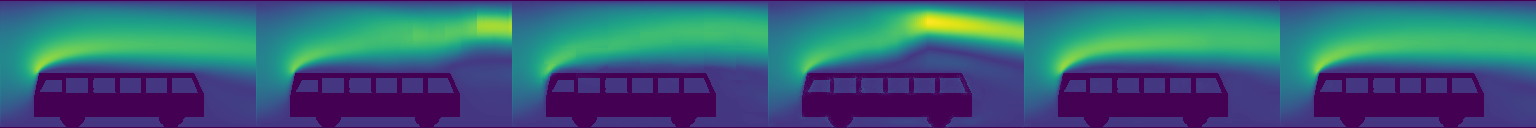
\includegraphics[width=0.82\textwidth]{./figures/data/pic_xin/final_8.png}
							\end{minipage}}
							\\
							\bottomrule
						\end{tabularx}
					\end{table}

表\ref{tab:total_comp_case}展示了基于不同深度学习方法预测的流场速度场的可视化结果。\textsc{FlowDNN} AP表示使用了注意力机制和神经网络剪枝的\textsc{FlowDNN}。
对于不同的汽车外形,\textsc{FlowDNN}的二维速度场预测结果都体现出与LBM求解器模拟结果的高度一致性。
观察\texttt{U-Net}和\texttt{T-Net}的预测结果,我们发现对于部分汽车外形如pickup(皮卡)和bus(公共汽车),
几何体上方的流场会出现明显的断层,原因可能是模型的泛化能力有限,对于不同的汽车外形的预测结果可能出现过拟合现象。
虽然\texttt{C-Net}对流场速度场的预测结果没有出现断层的现象,
但是可以看出速度场可视化结果模糊,这是预测结果精度不够导致的。
此外,\texttt{C-Net}预测结果具有明显的分块现象,这和\texttt{C-Net}在进行卷积操作时使用了较大的步长有关,
导致数据的局部性信息有较大程度的损失。



为了对不同深度学习方法的流场预测结果进行进一步分析,本文比较了不同深度学习方法的二维速度场预测结果与真值的差异。
如表\ref{tab:total_comp_case_error}所示,深度学习模型的预测误差主要集中在几何体周围以及几何体尾部区域。
这是由于流体绕物流动时会产生涡旋区,主要集中在几何体表面边界层。
这随着流动的进行,涡旋会与物体脱离,继而在物体后部形成不稳定带旋涡的尾流。
所以在几何体周围以及几何体尾部区域中,流体的运动规律更加复杂,导致模型预测误差较大。
对比\textsc{FlowDNN}和三个基线模型的预测结果与真值的差异,
可以直观地看出\textsc{FlowDNN}能够对二维速度场进行准确的预测,有效降低几何体周围以及几何体尾部区域的预测误差。




\begin{table}[htp]
	\caption{不同深度学习方法的二维速度场预测结果与真值的差异比较}
	\label{tab:total_comp_case_error}
	\centering
	\begin{tabularx}{14cm}{p{0.8cm}p{2cm}p{2cm}p{2cm}p{2cm}p{2.4cm}}
		\toprule
		&  ~~~~~~~\textit{U-Net} & ~~~~~~~\textit{C-Net} & ~~~~~~~\textit{T-Net} & ~~~\textit{FlowDNN} & ~~~\textit{FlowDNN AP}   \\
		\midrule
		
		racing &\multicolumn{5}{l}{
			\begin{minipage}{\textwidth}
				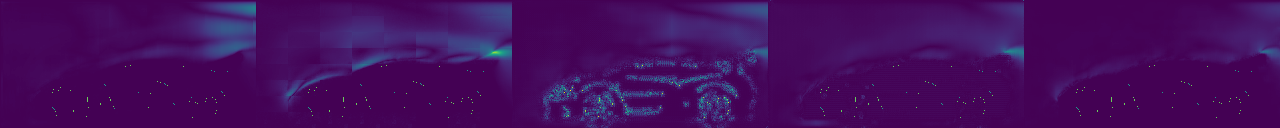
\includegraphics[width=0.82\textwidth]{./figures/data/pic_xin_error/final_35.png}
			\end{minipage}}
		\\
		
		saloon &\multicolumn{5}{l}{
			\begin{minipage}{\textwidth}
				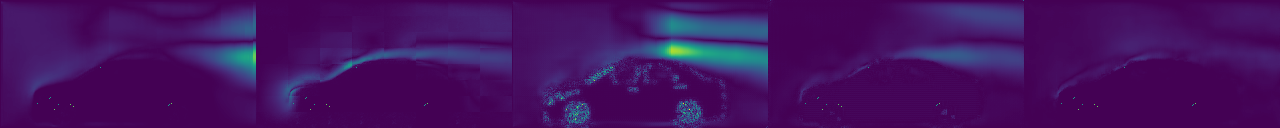
\includegraphics[width=0.82\textwidth]{./figures/data/pic_xin_error/final_32.png}
			\end{minipage}}
		\\
		jeep &\multicolumn{5}{l}{
			\begin{minipage}{\textwidth}
				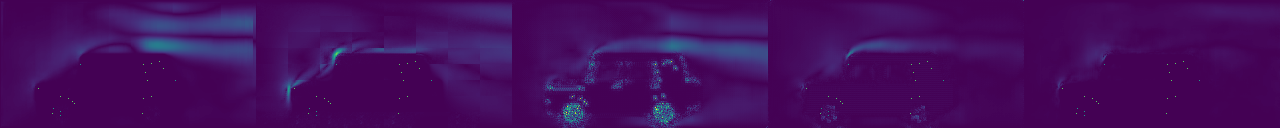
\includegraphics[width=0.82\textwidth]{./figures/data/pic_xin_error/final_20.png}
			\end{minipage}}
		\\
		pickup &\multicolumn{5}{l}{
			\begin{minipage}{\textwidth}
				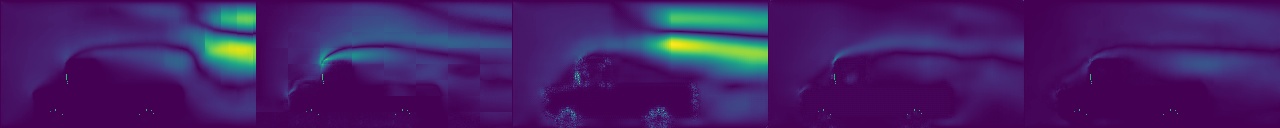
\includegraphics[width=0.82\textwidth]{./figures/data/pic_xin_error/final_39.png}
			\end{minipage}}
		\\	
		bus &\multicolumn{5}{l}{
			\begin{minipage}{\textwidth}
				
\includegraphics[width=0.82\textwidth]{./figures/data/pic_xin_error/final_8.png}
			\end{minipage}}
		\\
		\bottomrule
	\end{tabularx}
\end{table}


\subsubsection{物理损失函数}\label{phy_effect}

为了探究物理损失函数对流场预测结果的影响,尤其是对预测结果和CFD求解器模拟结果的物理一致性的影响,
本文分别使用$L_{physical}$和$L_{1}$损失函数对\textsc{FlowDNN}进行了训练。

\begin{figure}[htp]
	\centering
	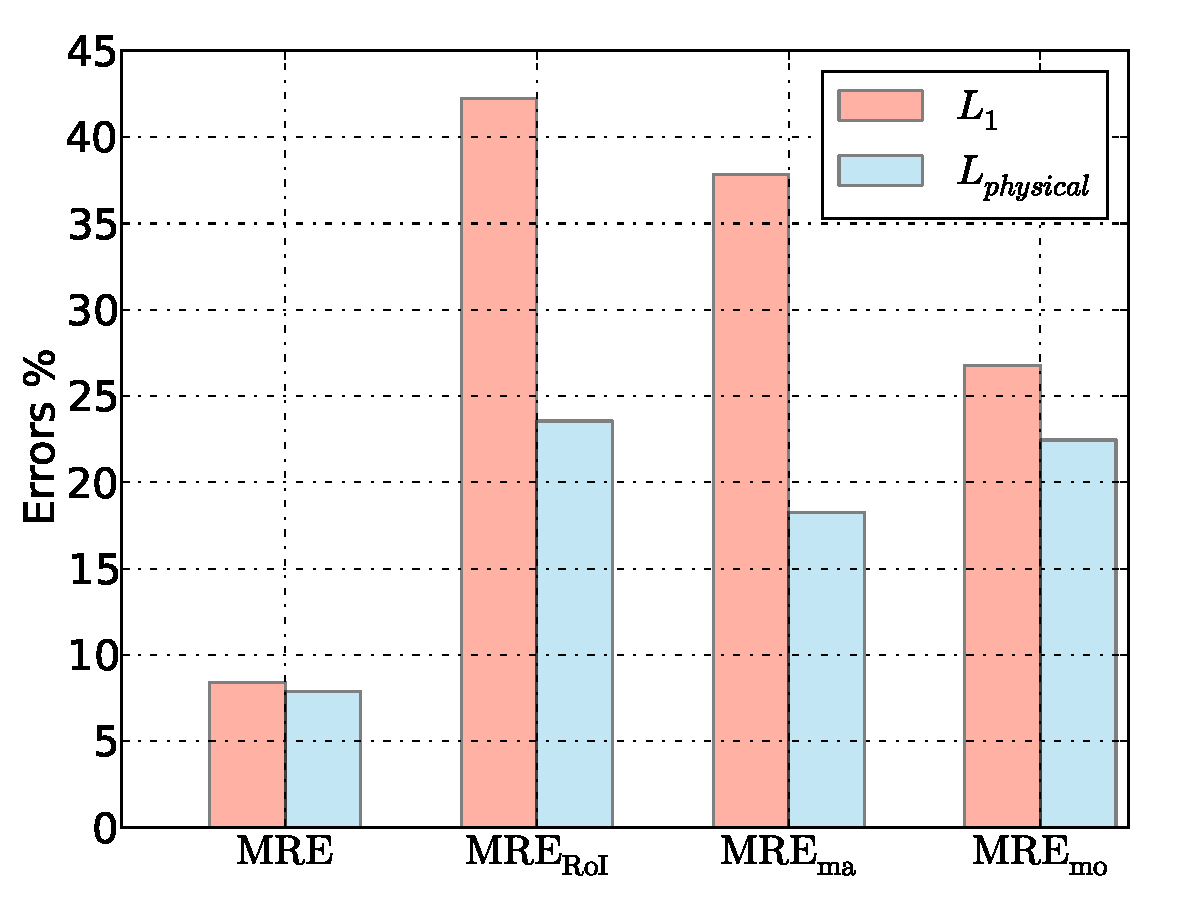
\includegraphics[width=0.58\textwidth]{./figures/data/data_pre/loss_comp.pdf}
	\caption{不同损失函数对流场预测结果的影响}
	\label{fig:phy_bar_comp}
\end{figure}

\noindent 图\ref{fig:phy_bar_comp}展示了不同损失函数在$MRE$、$MRE_{RoI}$、$MRE_{ma}$和$MRE_{mo}$四项性能指标的表现。
可以看到,相对于传统的$L_{1}$损失函数,使用物理损失函数训练预测模型可以有效地降低$MRE_{ma}$(从37.83\%降低至18.28\%),
质量守恒误差减小了一半。
物理损失函数对降低动量守恒误差$MRE_{mo}$也有一定效果,
我们分析$L_{physical}$对$MRE_{ma}$和$MRE_{mo}$影响不同的原因和损失函数权重有关。

我们对物理损失函数对预测结果的物理一致性的影响进行了进一步探究。
图\ref{fig:phy_hotmap}展示了真值和不同损失函数预测结果在每个格子点上质量和动量的变化值。
可以看出质量和动量的变化主要集中在定义的RoI区域和流场尾部区域,
这也导致了使用物理损失函数训练的流场预测模型,其预测结果的$MRE$并没有显著降低,
而$MRE_{RoI}$从42.23\%降低至23.56\%。
此外,我们观察到$L_{1}$的预测结果会出现不符合流体流动规律的情况,即$\Delta \mathrm{mass}$位于几何体内部,
物理损失函数可以有效减少这种情况的发生,增强预测结果和CFD求解器模拟结果的物理一致性。


\begin{figure}[htp]
	\centering
	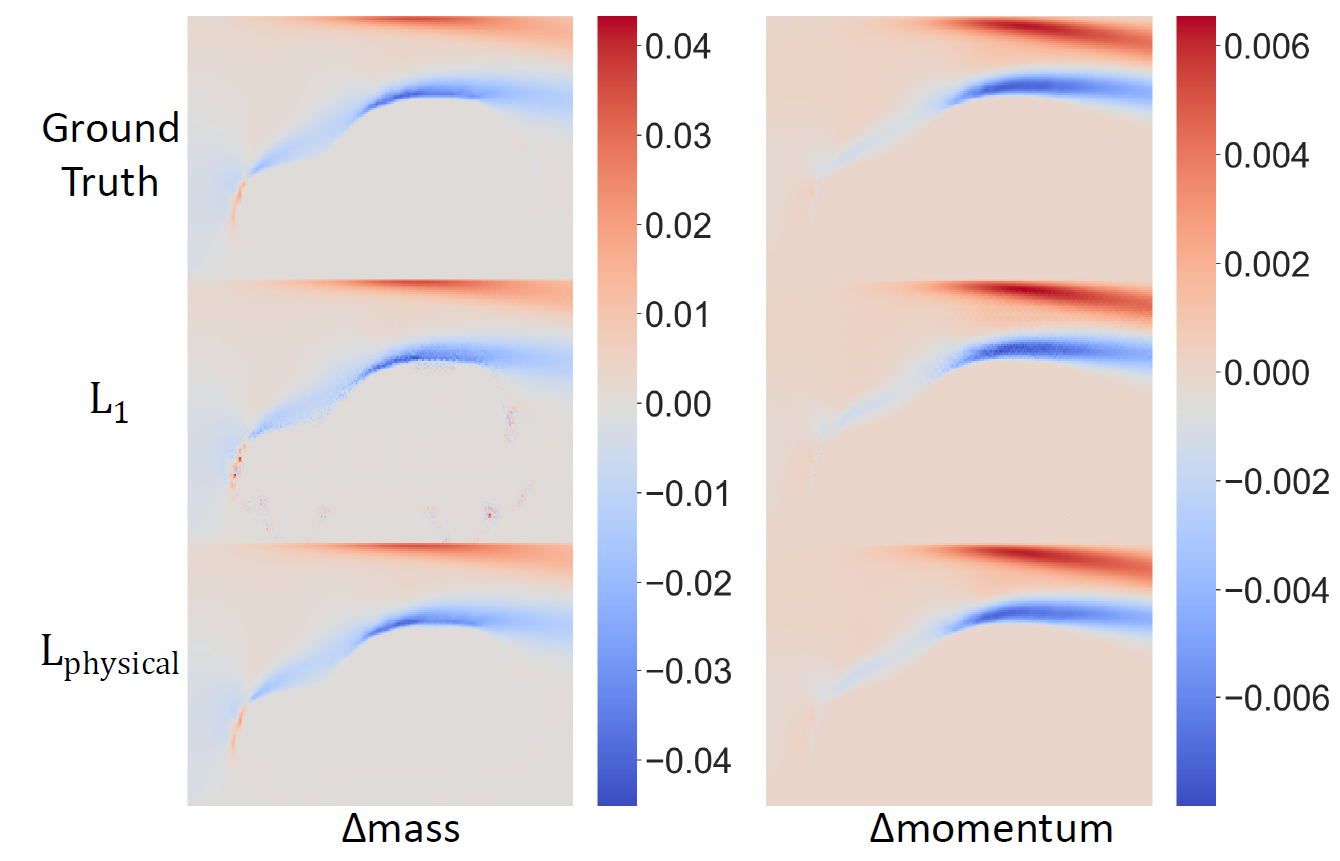
\includegraphics[width=0.62\textwidth]{./figures/data/loss_comp_case/loss_comp.png}
	\caption{不同损失函数对流场预测结果物理一致性的影响}	
	\label{fig:phy_hotmap}	
\end{figure}

\subsubsection{注意力机制}
为了提升模型的表示能力和非线性,提高\textsc{FlowDNN}对RoI区域的预测精度,
我们在\textsc{FlowDNN}的skip connections上嵌入了SAM和CAM模块。
从表\ref{tab:all_comp}中可知,嵌入注意力模块的\textsc{FlowDNN}有效增加了神经网络对RoI区域信息的提取能力,使RoI区域的平均相对误差$MRE_{RoI}$下降至9.16\%,同时提升了全场的预测准确率。
图\ref{fig:attention_violin}展示了在使用和不使用注意力模块的情况下,\textsc{FlowDNN}的$MRE_{RoI}$误差在测试集上的分布。
在未使用注意力机制之前,测试集上$MRE_{RoI}$误差集中在18\%左右;使用注意力机制之后,$MRE_{RoI}$误差集中在6\%左右,而且误差分布更加集中,提升了\textsc{FlowDNN}的流场预测稳定性。

\begin{figure}[htp]
	\centering
	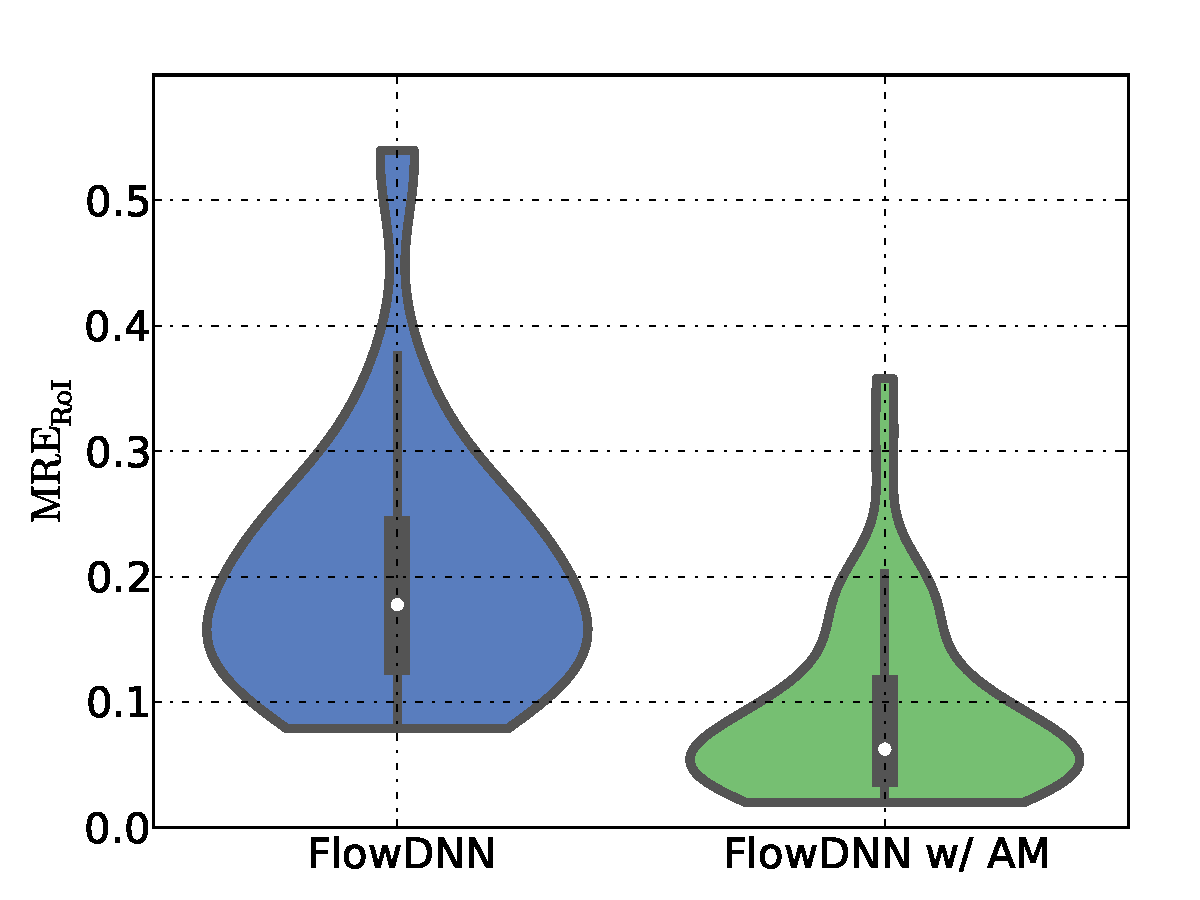
\includegraphics[width=0.58\textwidth]{./figures/data/data_pre/error_s_compare_violin.pdf}
	
	\caption{注意力机制对$\rm{MRE_{RoI}}$在测试集上分布的影响}
	\label{fig:attention_violin}
\end{figure}

图\ref{fig:attention_val_loss_comp}展示了注意力机制对预测模型训练的影响。
相比不使用注意力机制的情况,嵌入了CAM和SAM模块的\textsc{FlowDNN}随着训练的进行收敛地更快,
在50个epoch时验证上的损失函数已经收敛到较低的水平,在150个epoch时验证集上的误差已经趋于稳定。
对比两条曲线的振幅,嵌入注意力模块的蓝线在垂直方向上的振幅更小,模型训练过程更加稳定。
在两条误差曲线都趋于稳定时,使用注意力模块的\textsc{FlowDNN}的误差收敛至更低的水平。

\begin{figure}[htp]
	\centering
	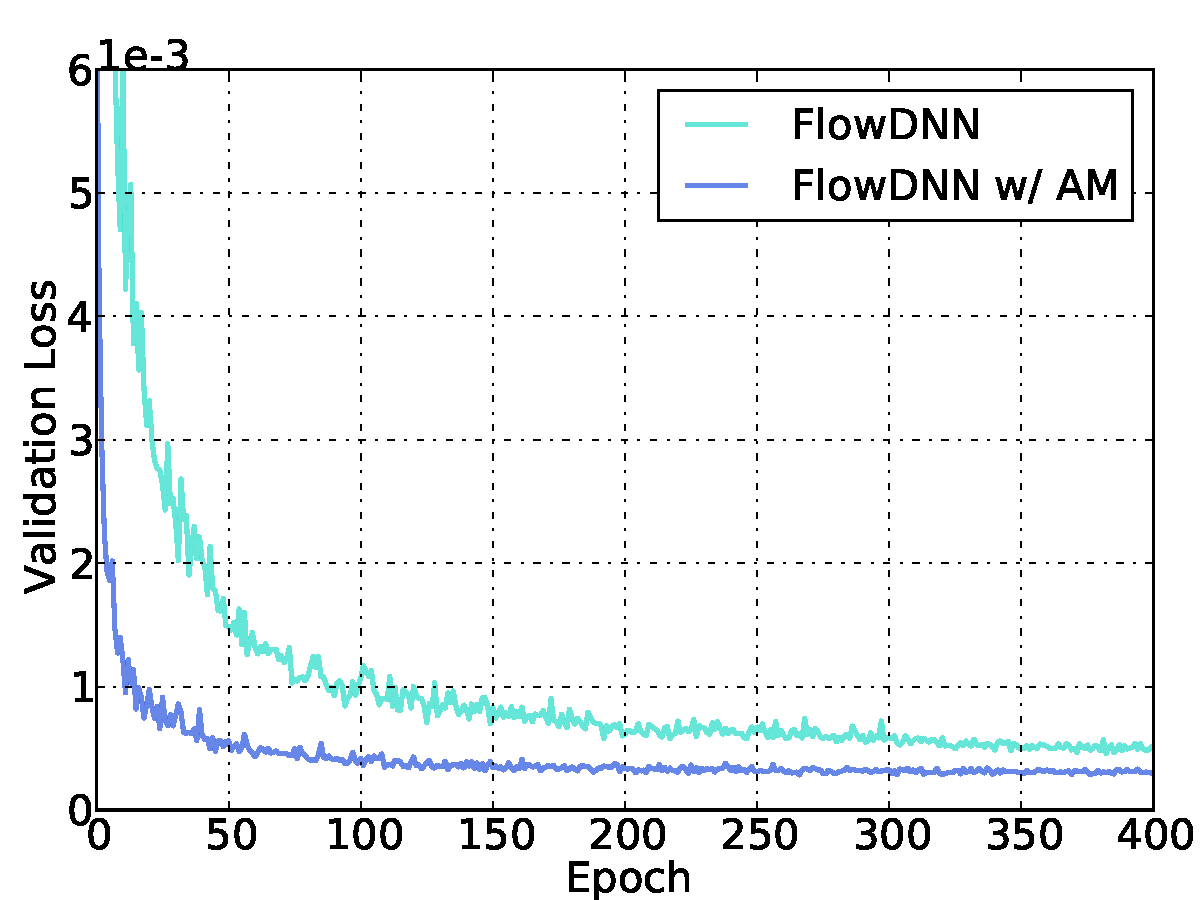
\includegraphics[width=0.58\textwidth]{./figures/data/am_comp.pdf}
	\caption{注意力机制对模型训练的影响}
	\label{fig:attention_val_loss_comp}
\end{figure}

由此可见,在\textsc{FlowDNN}中合理地嵌入注意力模块,不仅能大幅提升模型在RoI区域的预测精度,
还有助于加速模型训练收敛,缩短模型训练的时间,同时提高模型的预测稳定性。


\subsubsection{激活函数}\label{ac_effect}
激活层是深度神经网络的重要组成部分,对保证神经网络的非线性预测能力和提升神经网络模型的预测效果有重要影响。
本文比较了常用于气动预测模型的ReLU和ELU两种激活函数对气动流场预测模型的影响。
图\ref{fig:activation_intro}展示了两种激活函数的工作原理。

对ReLU激活函数有:
\begin{equation}
\varphi(x)=\max (0, x)
\end{equation}

\noindent 对ELU激活函数有:
\begin{equation}
\varphi(x)=\left\{\begin{array}{ll}
x & \text { if } x>0 \\
\alpha\left(e^{x}-1\right) & \text { if } x \leq 0
\end{array}\right.
\end{equation}

\noindent ReLU和ELU的x > 0 的部分作用效果是相同的,保留神经元的原始输入(y = x),都能有效克服梯度消失的问题\cite{2010Rectified};
在x < 0的部分,ReLU会将神经元的输出置为0,ELU则将输出映射到(-1,0)之间。


\begin{figure}[htb]
	\centering
	\subfloat[]{\label{fig:relu}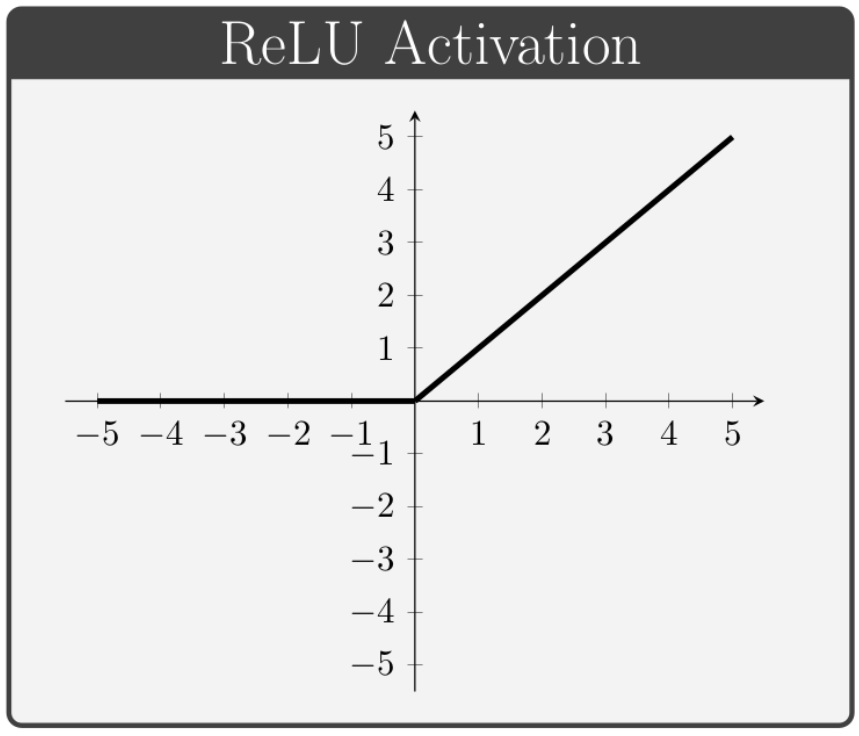
\includegraphics[width=0.38\textwidth]{figures/ReLU.png}} \qquad
	\subfloat[]{\label{fig:elu}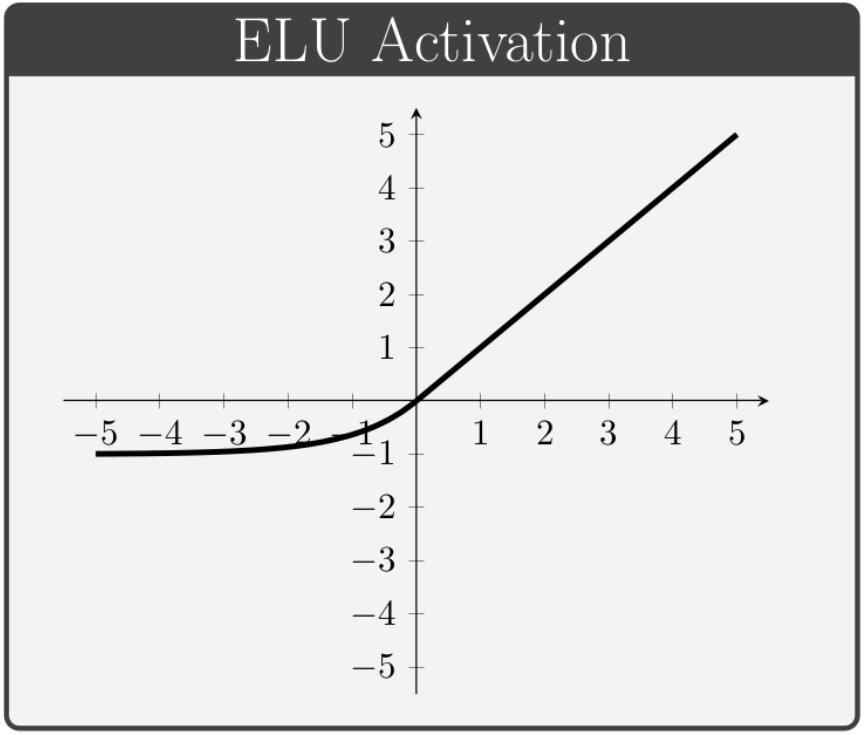
\includegraphics[width=0.38\textwidth]{figures/ELU.png}} 
	\caption{ReLU和ELU激活函数}
	\label{fig:activation_intro}
\end{figure}


图\ref{fig:activation}展示了ReLU和ELU两种激活函数对模型训练的影响。
为了保证模型收敛和避免模型训练产生梯度爆炸,
在激活函数进行处理之前我们对输入数据进行了批标准化(batch normalization,BN)。
在使用BN的情况下,使用ReLU作为激活函数模型随着训练收敛地更快;
训练稳定后,在测试集上的误差也小于使用ELU作为激活函数的情况。
我们分析ELU激活函数表现较差的原因可能是ELU本身能够将激活单元的输出均值往0推近,
和批标准化作用相似。所以ELU配合BN操作使用时,因为多次数据标准化处理,预测性能反而会较差。
因此我们对仅使用ELU激活函数的情况进行了测试,结果表明,仅使用ELU和ReLU+BN的效果相当。
考虑到ReLU激活函数能够将部分神经元输出置为0,增加神经网络的稀疏性,有利于神经网络剪枝,因此本章选取其作为激活函数。

\begin{figure}[htp]
	\centering
	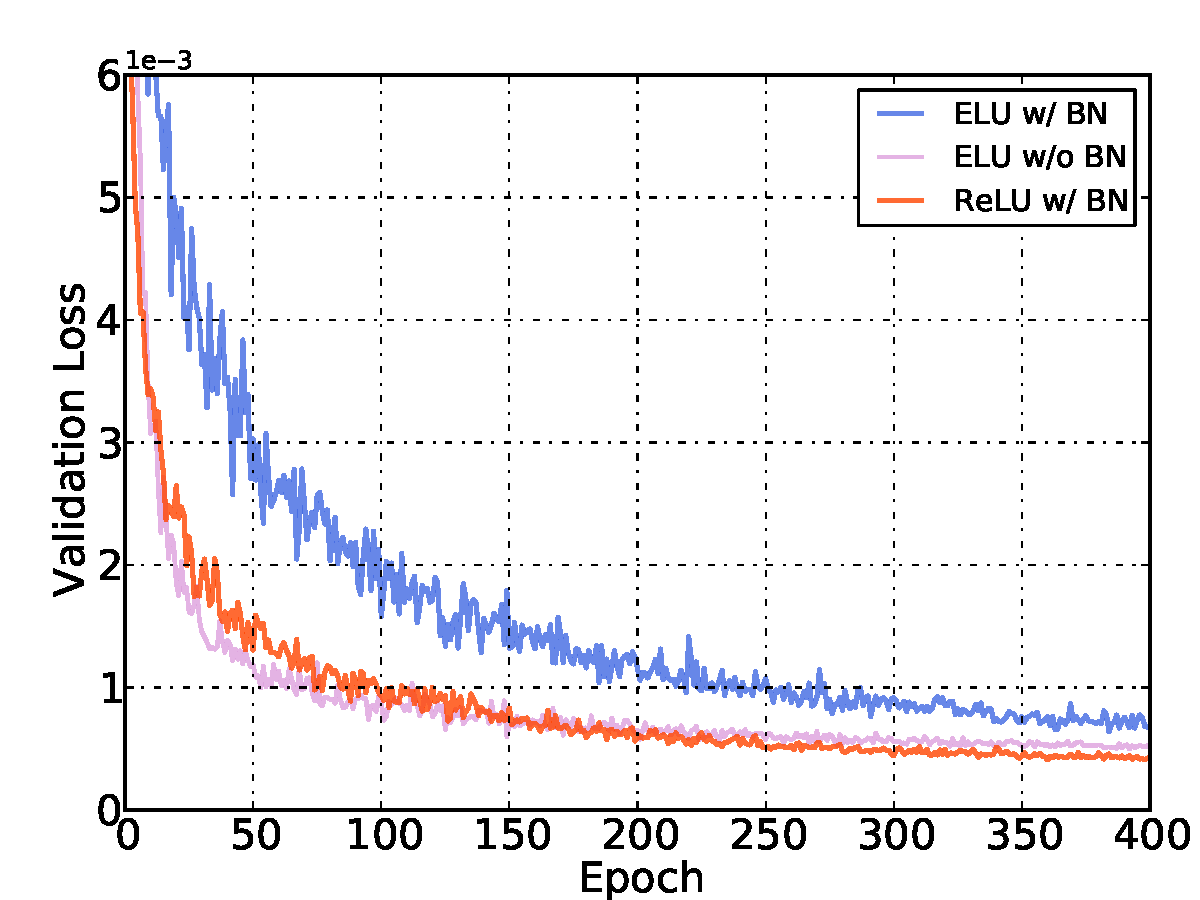
\includegraphics[width=0.58\textwidth]{./figures/data/activation_comp.pdf}
	\caption{不同激活函数对模型训练的影响}
	\label{fig:activation}	
\end{figure}


\subsubsection{神经网络剪枝}

在选定损失函数,利用注意力机制对\textsc{FlowDNN}进行优化之后,我们对\textsc{FlowDNN}进行了神经网络剪枝。
引入神经网络剪枝主要出于两方面的考虑:
一方面剪枝后的预测模型参数减少,可以证明\textsc{FlowDNN}的预测性能提升不是简单地增加参数量;
另一方面,通过神经网络剪枝精简网络结构,加快预测模型推理速度。

\begin{figure}[htp]
	\centering
	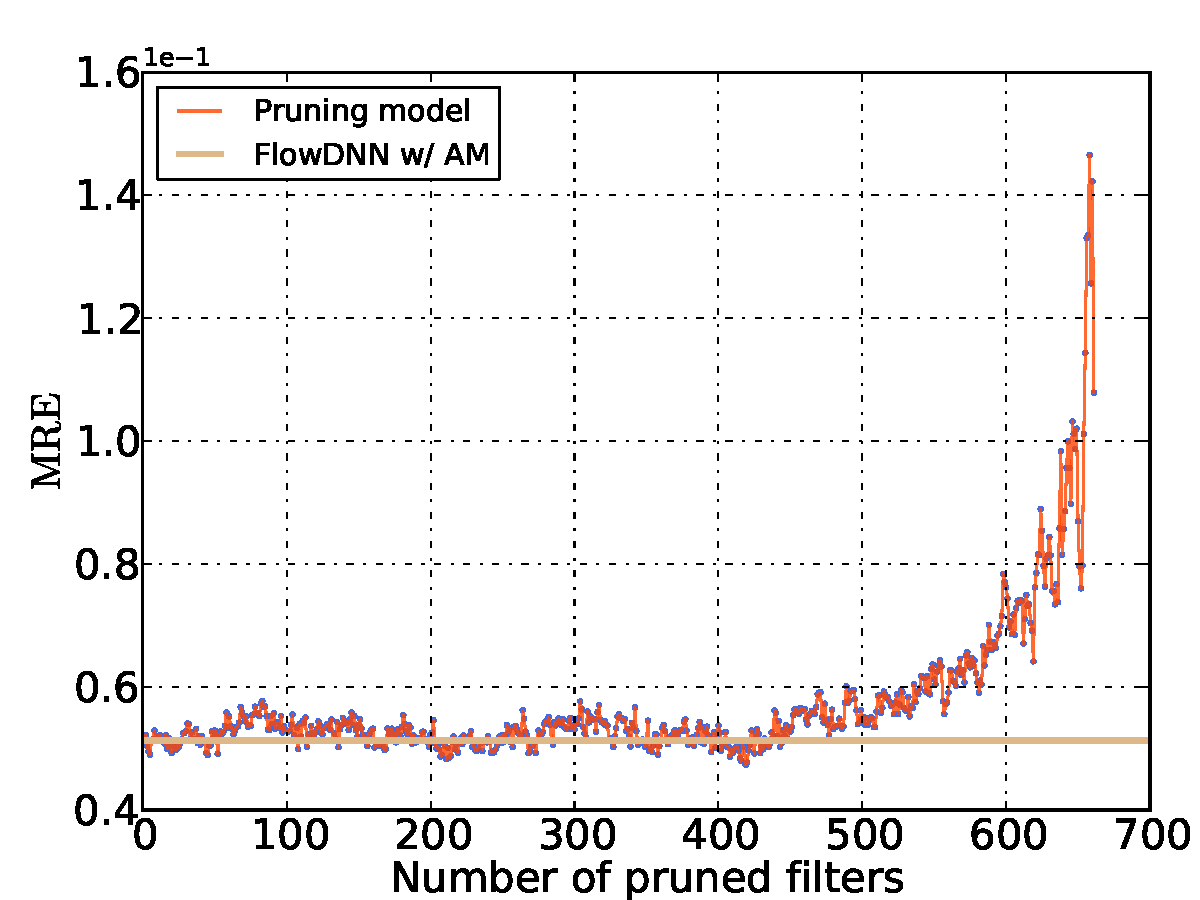
\includegraphics[width=0.58\textwidth]{./figures/data/pruning_result.pdf}
	\caption{网络剪枝对$MRE$的影响}
	\label{fig:pruning_result}	
\end{figure}

图\ref{fig:pruning_result}展示了神经网络剪枝对\textsc{FlowDNN}预测结果的平均相对误差的影响。
其中平行于坐标横轴的是剪枝前\textsc{FlowDNN}的MRE误差,随着剪枝的进行,模型的MRE误差一直在基线上下波动;
在剪枝神经元数量超过500之后,随着剪枝继续进行,破坏了神经网络结构,导致MRE误差急剧上升。
本文选取MRE误差最小的剪枝模型作为最终的气动流场预测模型,整个二维速度场预测结果的平均相对误差仅为4.77\%。


\section{本章小结}

本章针对传统CFD方法进行流场模拟效率低的问题,
提出一种基于深度卷积网络的端到端流场预测方法。
首先分析了基于深度卷积网络进行流场预测的优势,对比了流场模拟任务和传统图像转换任务的相似点与不同点。
其次研究了基于笛卡尔网络的流场数据表示方法,包括SDF方法和二元法。
然后提出了基于U-net网络的气动流场预测模型\textsc{FlowDNN},具体包括:
针对流体运动特点,通过改进U-net网络架构;
基于流体流动的物理规律,提出融合物理损失项和传统$L_1$损失项的物理损失函数;
针对边界层等RoI区域预测准确率低的问题,引入注意力模块;
通过神经网络剪枝进一步优化模型预测效率。
最后定义了新的流场预测结果评价指标,与传统CFD求解器和三个基线模型进行了全面的性能比较。

实验表明,相对于三个基线模型,\textsc{FlowDNN}在测试集上的全场预测准确率、RoI区域准确率更高,
预测结果与CFD模拟结果的物理一致性更高;
与基于LBM的传统CFD方法相比,流场模拟效率提升14000x,同时将预测误差控制在5\%以内。


